\documentclass[a4paper,10pt,twocolumn]{article}

\usepackage[utf8]{inputenc}
\usepackage[T1]{fontenc}
\usepackage{verbatim} 
\usepackage{fullpage}
\usepackage{xcolor,graphicx}
\usepackage[french, english]{babel}
\usepackage{indentfirst}
\usepackage{fancyvrb}
\usepackage{comment}


\newenvironment{code}
  {\fontfamily{pnc}\selectfont}{}
%pbk
%phv

\author{Colas Decron, Camille Le Roi}
\title{\centering Extension de Guido à la notation musicale contemporaine}

\date{ Février-Aout 2013}

\begin{document}

\selectlanguage{french}

\maketitle

\begin{abstract}

La librairie GUIDO offre un grand nombre de symboles musicaux correspondant aux plus larges besoins de l'écriture musicale. Elle fournit un moteur de rendu de partitions embarquable dans d'autres applications. Dans une volonté d'étendre cette librairie à la musique contemporaine, nous avons implémenté un ensemble de nouvelles notations jusqu'à présent pas, ou très sommairement, implémentées. L'objectif était de répondre aux demandes des compositeurs en ajoutant certaines notations de la manière la plus adaptée à l'écriture musicale, tout en laissant une large liberté à l'utilisateur.

\end{abstract}

\section{Introduction}

% format
% librairie
% compos
% état de l'art de la notation contemporaine
% pb de la notation contemporaine
% 
% Studying Music is Difficult and Important, Donald Byrd
% Music Notation Software and Intelligence, Donald Byrd
% A Brief Survey of Music Representation Issues Techniques and Systems
% Les logiciels d'aide à la composition musicale



Le format de notation musicale GUIDO (GMN) \cite{ref6} \cite{ref5} a été défini par H. Hoos et K. Hamel il y a plus de 10 ans. Il est très proche du format adopté par Lilypond \cite{ref7} mais il est apparu antérieurement. Le format GMN est un langage textuel de représentation de partitions musicales %. Il est basé sur un formalisme simple mais puissant, se concentrant sur les grands concepts musicaux (en opposition aux caractéristiques graphiques). L'approche développée par GUIDO repose sur l'idée d'adéquation, qui invite à noter simplement les concepts musicaux simples, et à ne recourir à des notations complexes que pour les notions musicales complexes.
sur lequel est basée %sur le format GMN, 
la librairie GUIDO \cite{ref5}. Cette dernière %fournit un puissant moteur de mise en page de partitions, qui 
se différencie notamment des approches de type compilateur par sa capacité à être embarquée dans une application indépendante, et par la rapidité et l'efficacité du moteur de rendu, qui le rendent utilisable dans un contexte temps réel pour des partitions simples.

\section{Format de Notation Guido}

%\subsection{Concepts de base}

Le format de base de GUIDO recouvre les notes, silences, altérations, voix indépendantes, et les concepts les plus courants de la notation musicale comme les clefs, métriques, armures, articulations, liaisons, etc.
Les notes sont représentées par leur nom, une altération optionnelle, un numéro d’octave optionnel et une durée optionnelle. Les accords sont décrits par des notes entre accolades séparées par des virgules. Un système (d'une ou plusieurs portées) est décrit par deux accolades, et une portée par deux crochets.

%\subsection{Tags GUIDO}

Les tags sont utilisés pour donner des informations musicales supplémentaires, comme les liaisons, clés, armures, etc. Un tag a une des formes suivantes : 

\begin{code}
\textbackslash{}tagname\textless{}param-list\textgreater{}

\textbackslash{}tagname\textless{}param-list\textgreater{}(note-series)
\end{code}

où param-list est une liste de paramètres (chaînes de caractères ou nombres), et où note-series est l'ensemble des notes ou accords concernés par le tag, dans le cas d'un range tag (tag possédant une durée).

\section{Implémentation de nouvelles notations}

%*****************TRILLES********************
\subsection{Trilles}

\begin{code}
\textbackslash{}trill\textless{}options\textgreater{}( accords )
\end{code}
\\

% littérature
% lilypond : e\trill f\trill ... sans vaguelette sinon \startTrillSpan ... \stopTrillSpan
%\gardner Read

Dans la version précédente, le trille à proprement parler n'était indiqué que par le symbole \textit{\textbf{tr}} placé au dessus de la note. Il paraissait pourtant important que la notation comprenne également la ligne ondulée du trille qui suit celui-ci et en indique la durée.

La question était alors de savoir jusqu'à quelle position devait se dessiner cette ligne, ainsi que les éventuelles variantes ou libertés données à l'utilisateur, et leur signification. En effet, comme ce symbole était déjà en partie implémenté, il fallait pouvoir lui offrir plus de souplesse sans pour autant en complexifier la notation.

D'après le livre "Behind Bars" d'Elaine Gould \cite{ref2}, la ligne du trille doit être dessinée depuis le signe \textit{\textbf{tr}} jusqu'au début du prochain évènement (la prochaine note ou le prochain soupir), sauf si celui-ci se situe directement après la prochaine barre de mesure, la ligne s'arrêtant dans ce cas à la barre elle-même. 

\begin{figure}[h]
\centering
\begin{code}
\{
[ \textbackslash{}meter\textless{}"2/4"\textgreater{} \textbackslash{}trill( \{a\} \{a/2\} ) ],

[ \textbackslash{}meter\textless{}"2/4"\textgreater{} \textbackslash{}trill( \{a\} \textbackslash{}tie( \{a\} \{a\} )) ]
\}
\end{code}
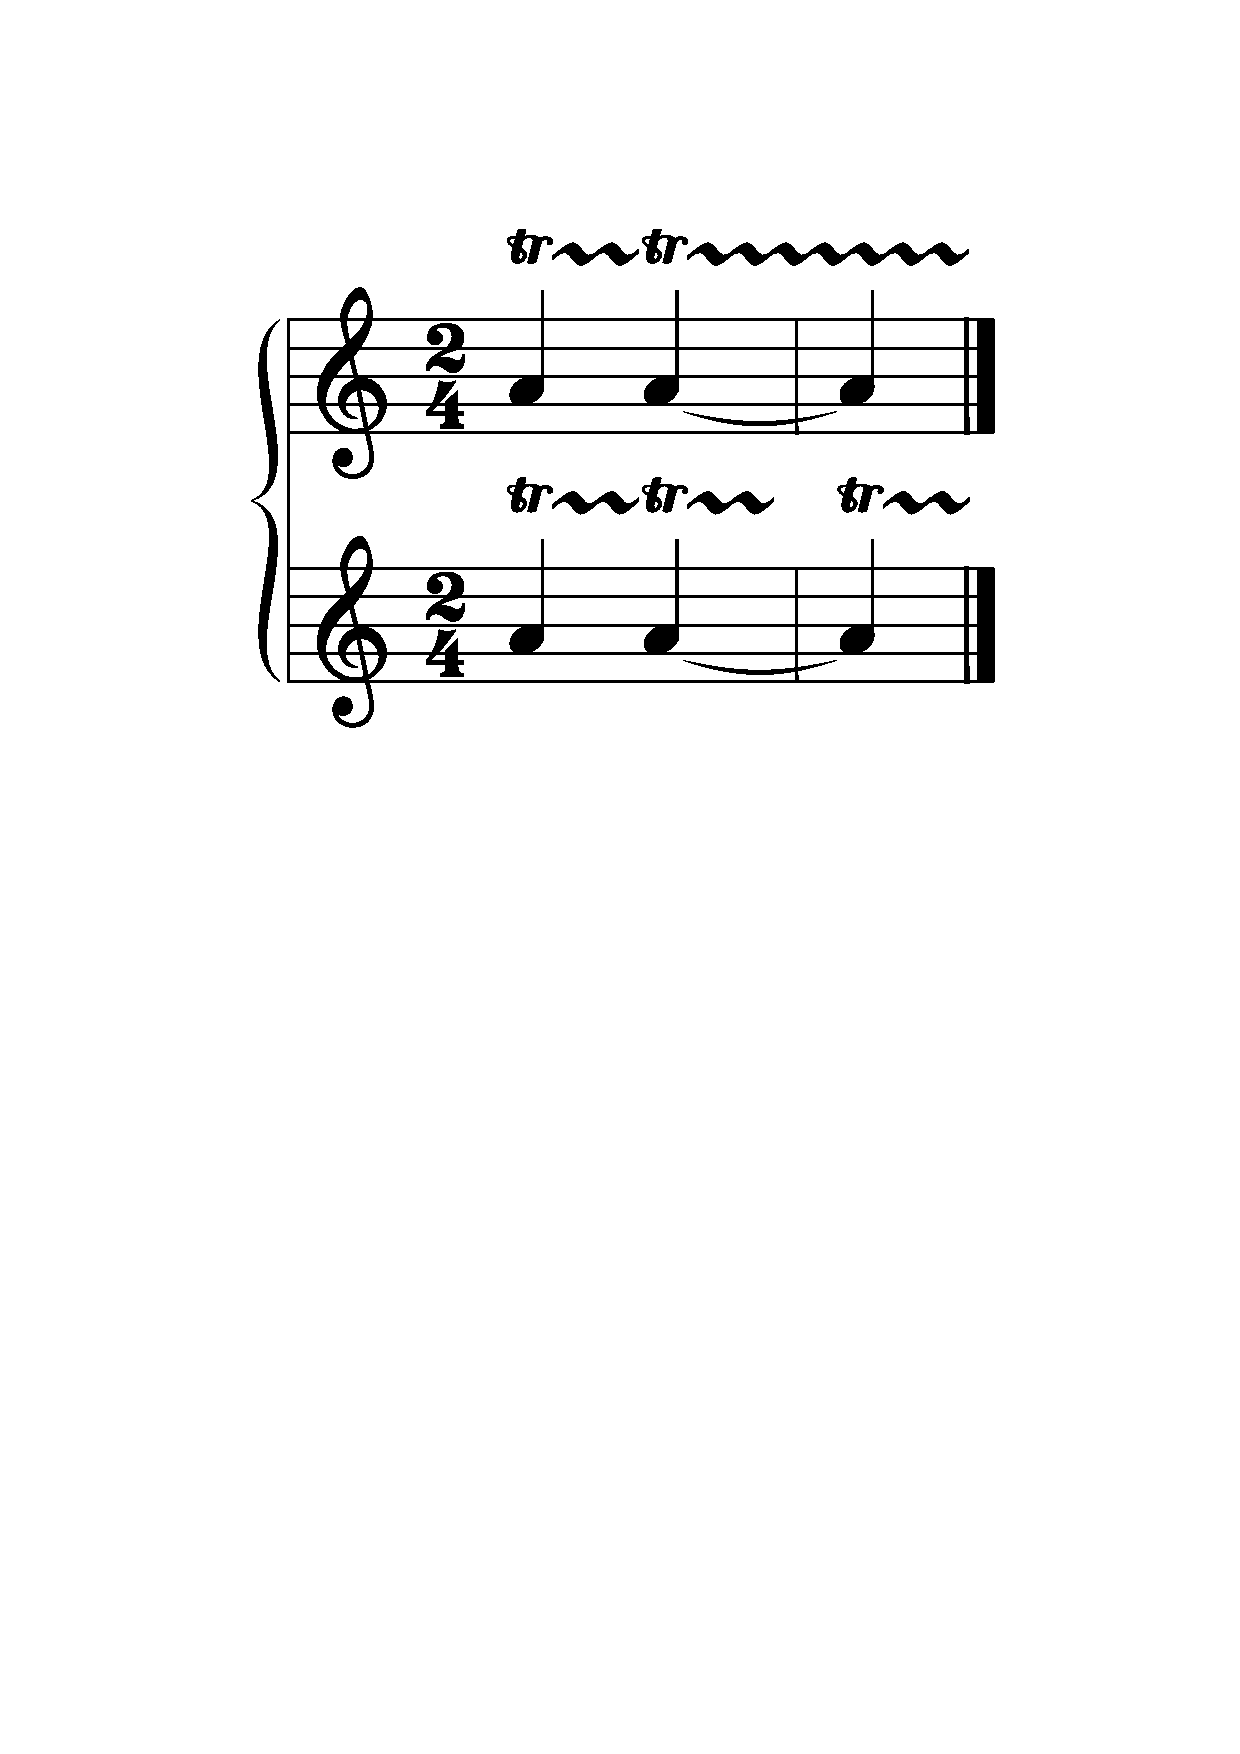
\includegraphics[width=6cm]{img/trill.pdf}
\caption{Cas du trille appliqué à des notes liées}
\label{fig:trill}
\end{figure}

Il fallut également définir le comportement quant aux notes liées, soit de manière automatique de par la présence d'une barre de mesure, soit de manière explicitement décrite par l'utilisateur. La solution adoptée est de dessiner la ligne de trille jusqu'à la fin de la dernière note liée si celle-ci provient d'une note plus longue découpée automatiquement, mais de s'arrêter normalement à la prochaine note si la liaison a été explicitée par l'utilisateur, qui pourra alors décider de répéter le trille sur cette autre note, ou non. (Figure \ref{fig:trill})

% justifier l'intérêt de tr et anchor ?
De plus, nous avons voulu donner la possibilité de choisir de dessiner ou non le signe \textit{\textbf{tr}}, ainsi que de pouvoir changer l'ancrage de la ligne pour le déplacer sur la tête de la note. Cela fut implémenté grâce aux options \textit{anchor} qui accepte comme valeurs "note" ou "tr" et \textit{tr} qui accepte comme valeurs "true" ou "false" (Figure \ref{fig:trillanchor}). Le reste des modifications graphiques pouvant être effectuées manuellement par l'utilisateur à travers les paramètres classiques de déplacement (\textit{dx}, \textit{dy}), de couleur (\textit{color}), et de taille (\textit{size}).

\begin{figure}[h]
\centering
\begin{code}
[ \textbackslash{}trill\textless{}tr="false", anchor="note"\textgreater{}( \{g\} \{a/2\} ) ]
\end{code}
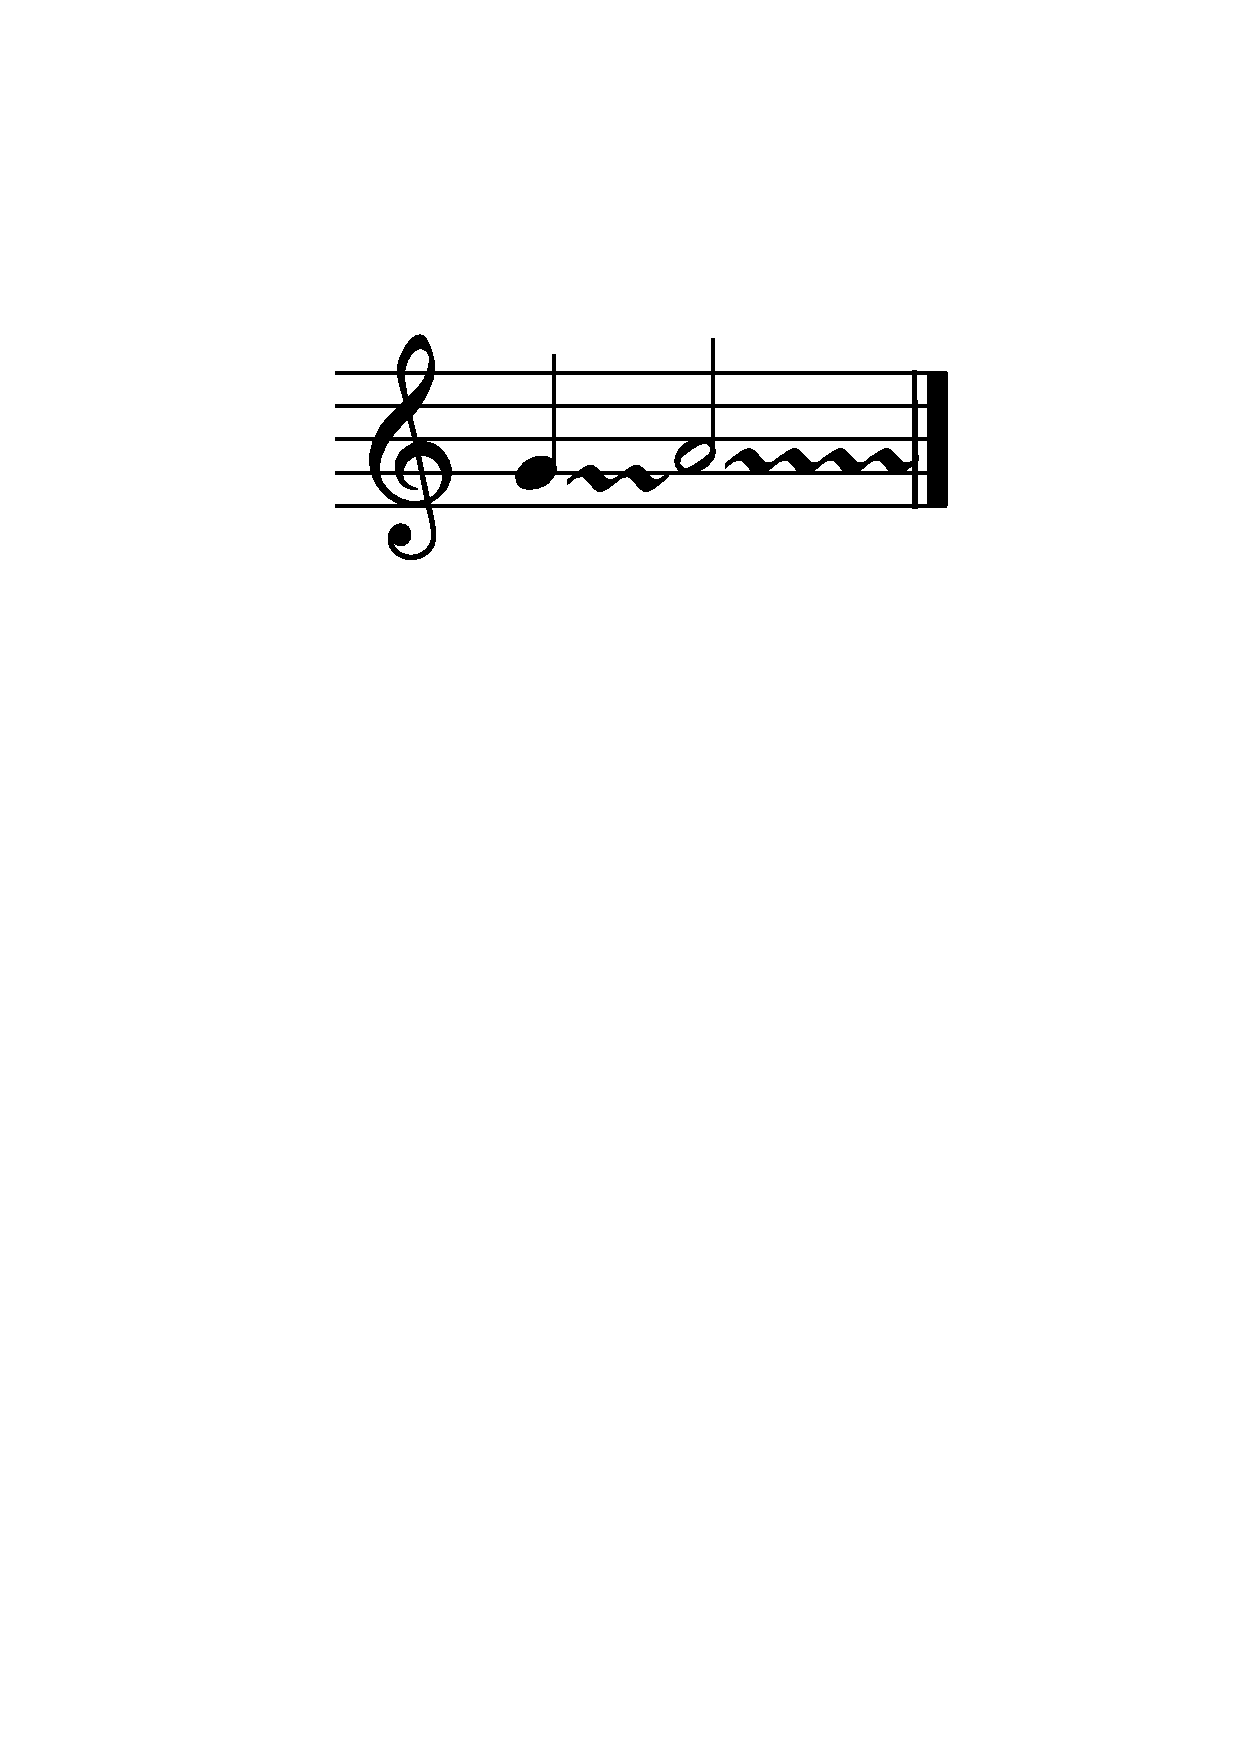
\includegraphics[width=5cm]{img/trillanchor.pdf}
\caption{Cas du trille ancré à la tête de note, et \textit{\textbf{tr}} optionnel}
\label{fig:trillanchor}
\end{figure}

\newpage

%**************TETES DE NOTES*********************
\subsection{Têtes de notes}

% colas //////////////////

\newpage

%*****************CLUSTERS*************************
\subsection{Clusters}

% colas /////////////////

\newpage

%***************GLISSANDO************************
\subsection{Glissandi}

\begin{code}
\textbackslash{}glissando\textless{}options\textgreater{}( notes )
\end{code}
\\

Dans un souci d'efficacité, il fallait pouvoir décrire un glissando seul ou plusieurs glissandi à la suite de la manière la plus simple et intuitive possible. 

Il paraissait important de donner la possibilité à l'utilisateur de n'écrire qu'une seule fois le tag pour décrire plusieurs glissandi consécutifs, contrairement à la description de lilypond où le tag doit être répété entre chaque note. Ainsi le range tag (tag possédant une durée) apparaissait comme la meilleure solution pour décrire un ou plusieurs glissandi : toutes les notes comprises dans les parenthèses seraient prises en compte et liées les unes aux autres par des glissandi. L'algorithme de démultiplication d'un même tag et de répartition de celui-ci est fortement inspiré de celui du tie, ou liaison de prolongation, qui doit également créer une liaison entre chacune des notes affectées.

Un choix devait également être fait quant à la répartition d'un glissando entre les différentes notes de deux accords, ne possédant eux-mêmes pas forcément le même nombre de notes. La solution proposée est celle qui nous a paru la plus intuitive : l'utilisateur choisit quelle note du premier accord sera liée avec quelle note du second. Pour ce faire, il lui suffit de les écrire dans l'ordre, c'est à dire : la première note de l'accord A sera liée à la première note de l'accord B, la seconde de A à la seconde de B\dots (Figure \ref{fig:glissandosimple})

\begin{figure}[h]
\begin{center}
\begin{code}
[\textbackslash{}glissando(\{e,a\} \{f,b\} \{a,d\})]
\end{code}

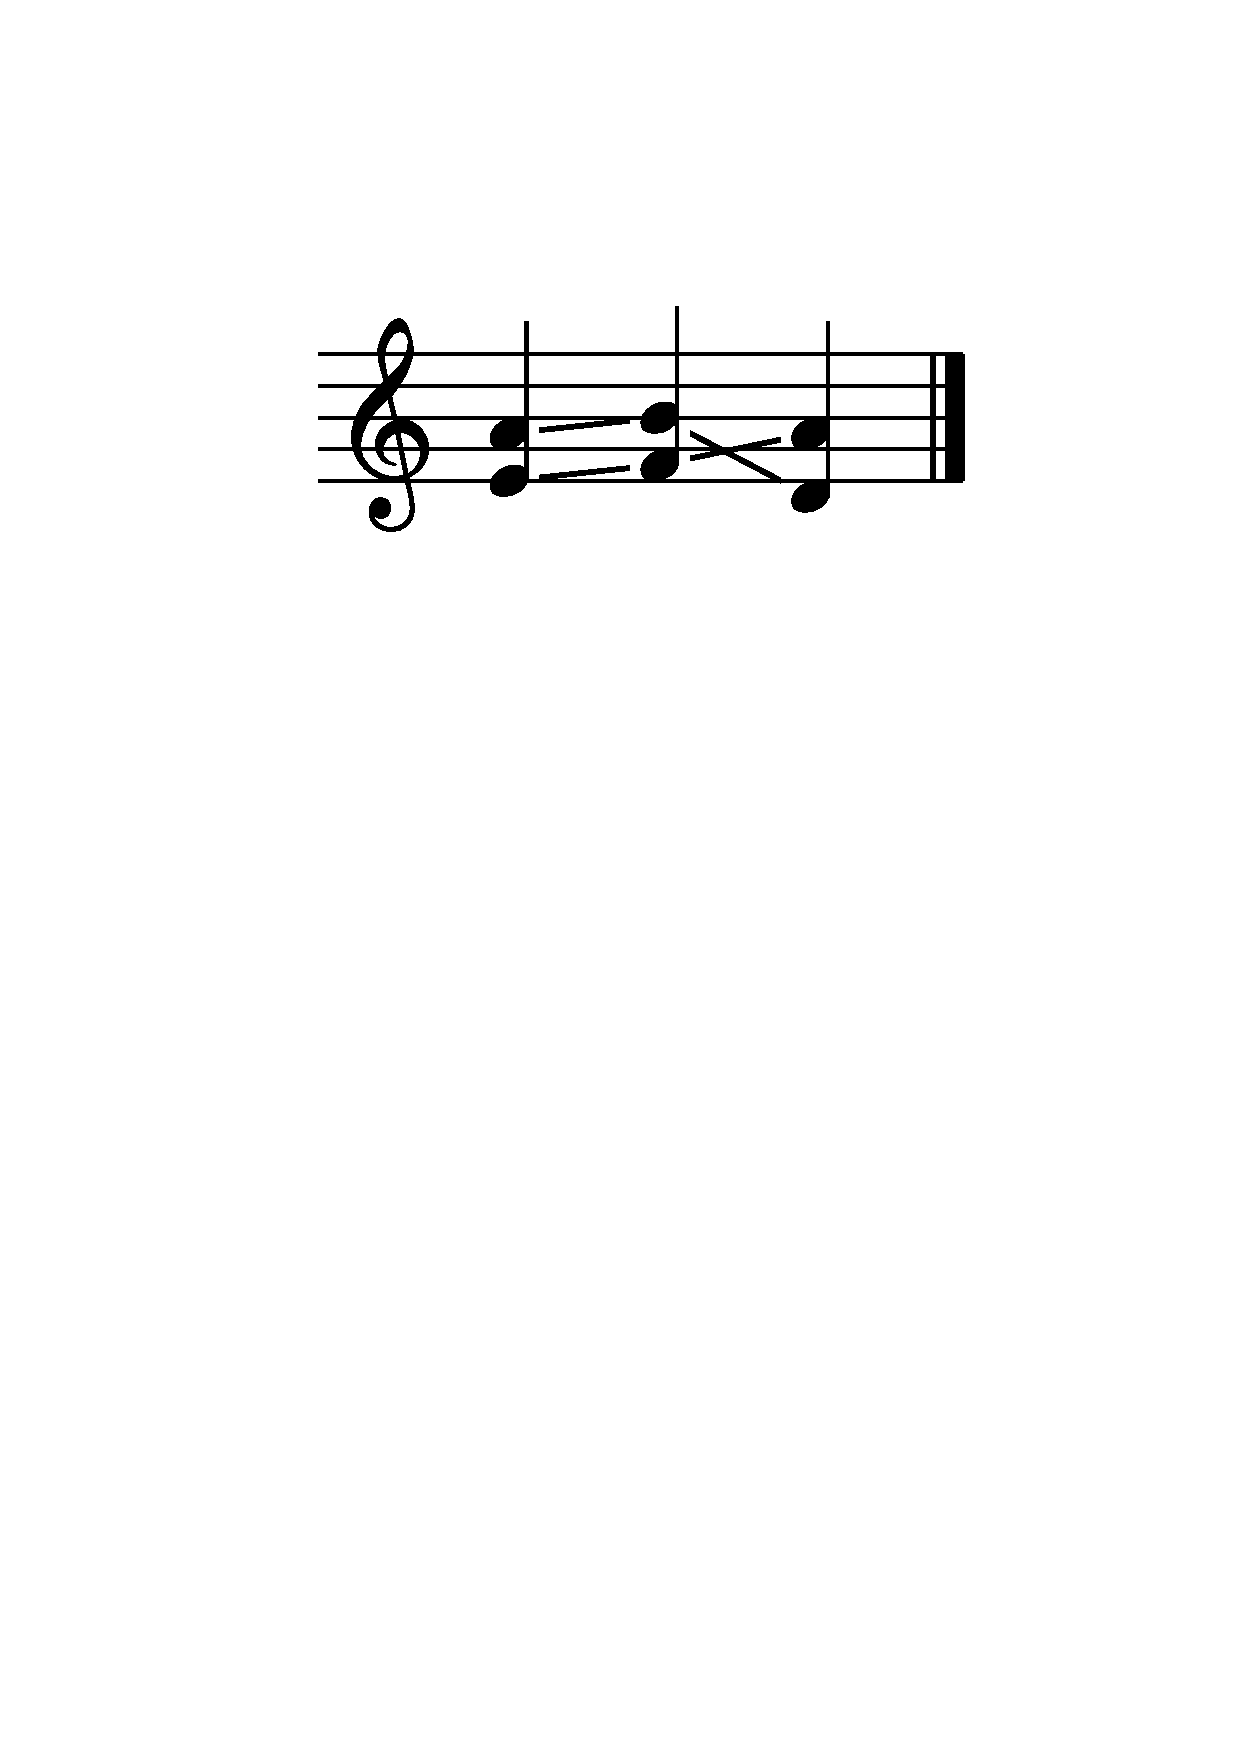
\includegraphics[width=5cm]{img/glissandosimple.pdf}
\caption{glisandi entre accords}
\label{fig:glissandosimple}
\end{center}
\end{figure}

L'unique problème avec ce choix peut se poser lors d'un conflit dans l'ordre imposé par le glissando précèdent et par le suivant, comme dans l'exemple Figure \ref{fig:glissando} . Il est alors possible de faire appel à une seconde voix, et au tag \textbackslash{}staff \textless{}\textit{numero de portée}\textgreater{} qui pourra créer sur une même portée d'autres glissandi en parallèle et indépendants des premiers.


\begin{figure}[h]
\centering
\begin{code}
[ \textbackslash{}glissando(e \{d,f,a\} g) b ]
\end{code}
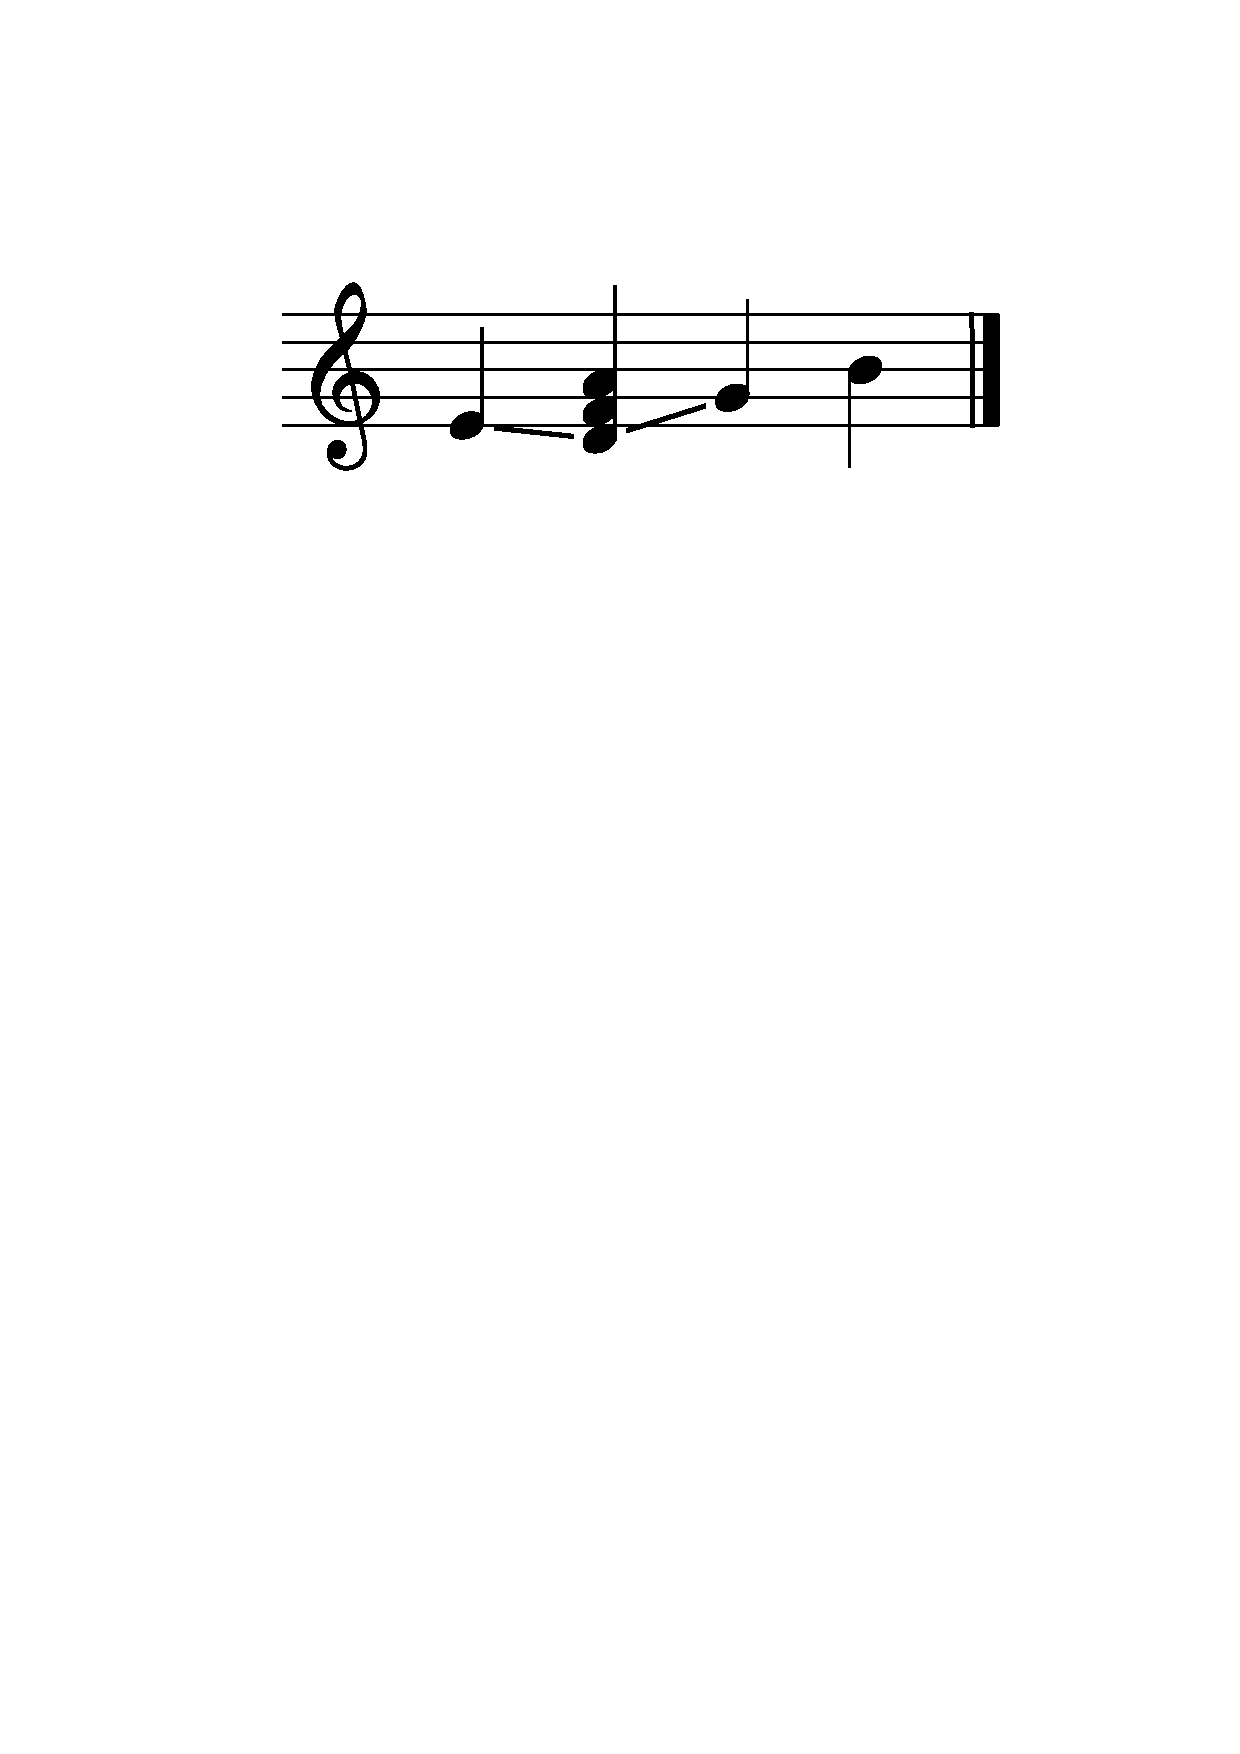
\includegraphics[width=55mm]{img/glissandopb.pdf}

\begin{code}
alors que l'on souhaite :
\end{code}
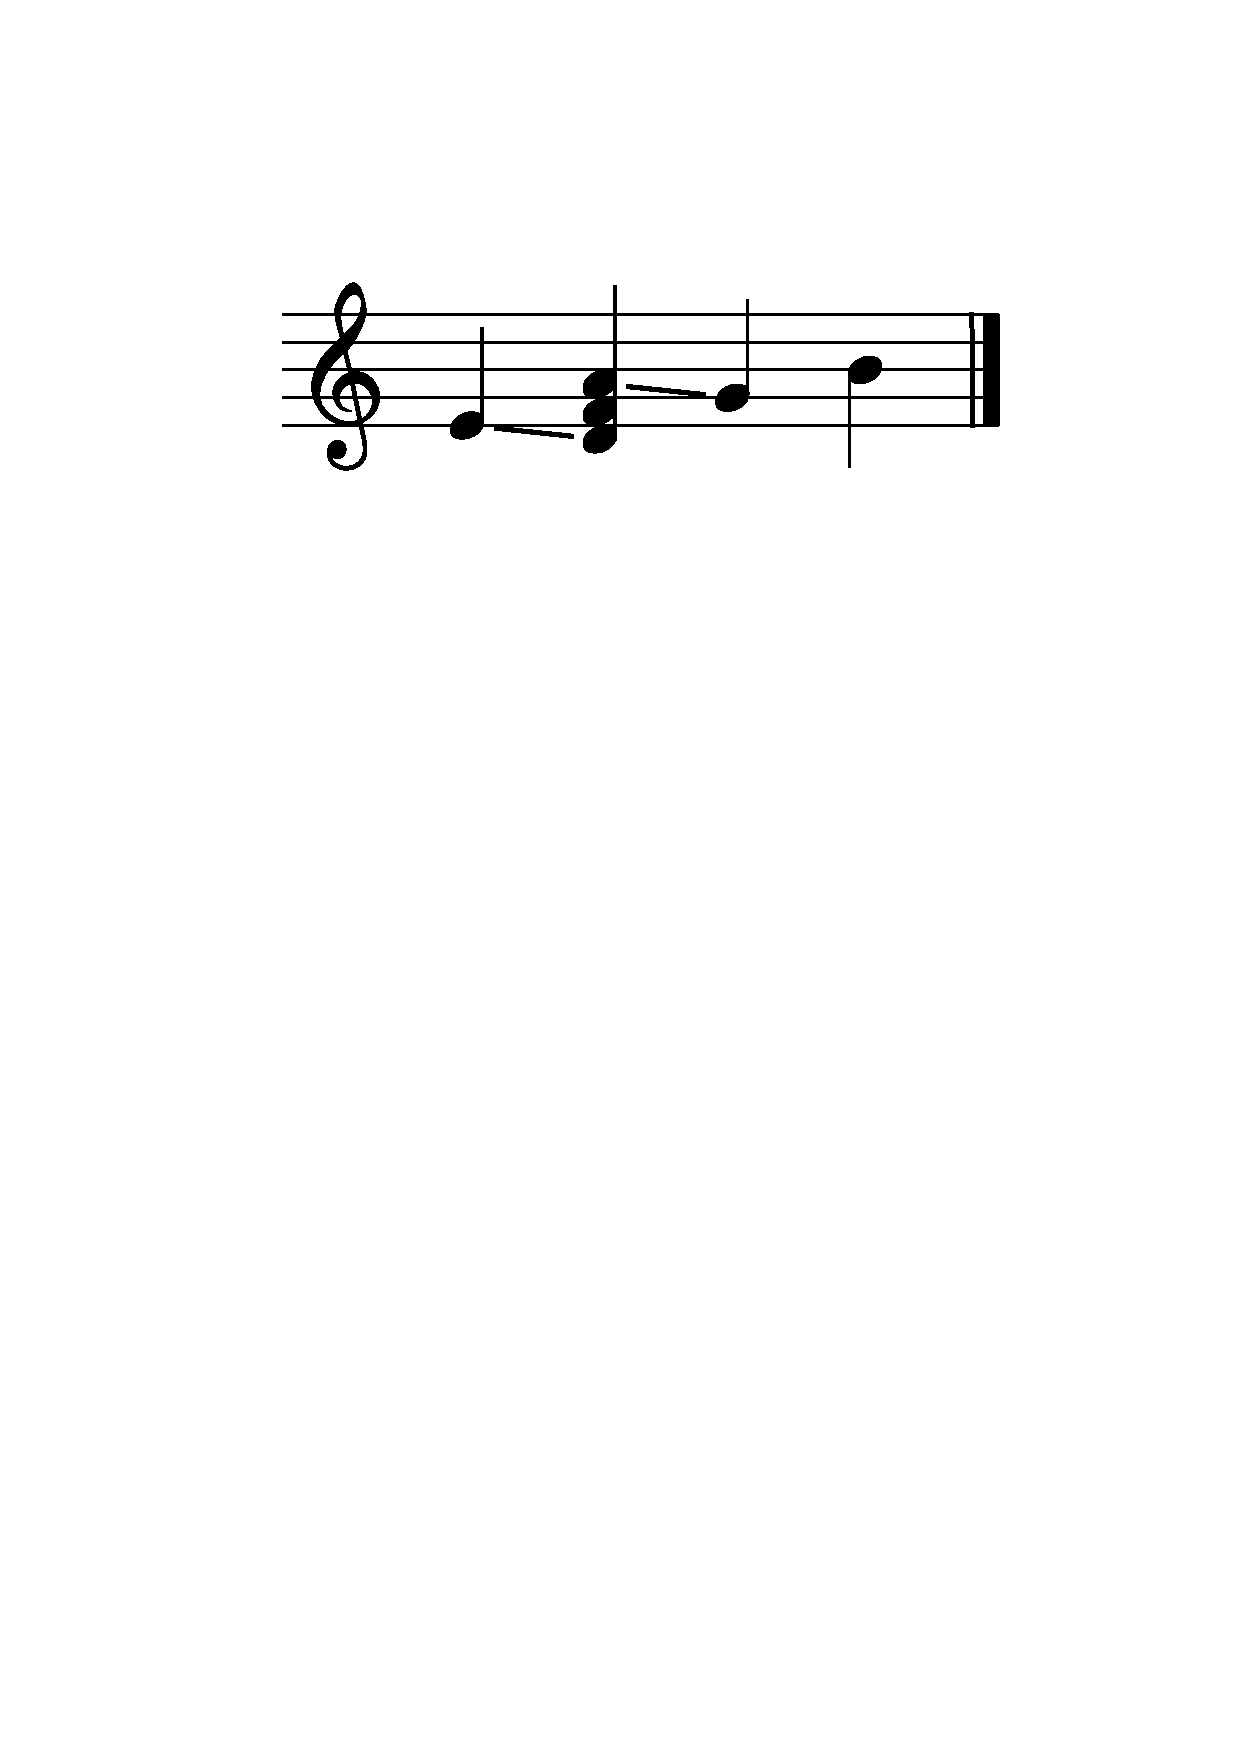
\includegraphics[width=55mm]{img/glissandosanspb.pdf}
\\
\begin{code}
\{ [ \textbackslash{}glissando( e \{d,f\}) empty b ],

[ \textbackslash{}staff\textless{}1\textgreater{} empty \textbackslash{}glissando( a g ) empty ] \}
\end{code}
\caption{Cas de recours à une seconde voix pour le glissando -
\textit{'empty' représente une note vide}}
\label{fig:glissando}
\end{figure}

Enfin, dans le cas d'accords ou de clusters, et donc de plusieurs glissandi simultanés, il nous a paru intéressant, comme on peut le voir dans "Behind Bars" p.143 \cite{ref3} ou dans "Music Notation in the Twentieth Century" p.61 \cite{ref2}, de donner la possibilité de remplir l'espace entre ces glissandi grâce à une option "fill". Une certaine flexibilité peut être trouvée dans le dessin grâce aux options graphiques dx1, dx2, dy1, dy2, ainsi que thickness qui permettent de modifier l'aspect du glissando. (Figure \ref{fig:glissandofill})

\begin{figure}[h]
\begin{center}
\begin{code}
[ \textbackslash{}glissando\textless{}fill="true", dx1=-2, dx2=2, thickness=2.2\textgreater{}(\textbackslash{}cluster(\{e,g\} \{c,b\}))
\textbackslash{}glissando\textless{}fill="true"\textgreater{}(\{c,e,g\} \{a,c2,f1\}) ]
\end{code}

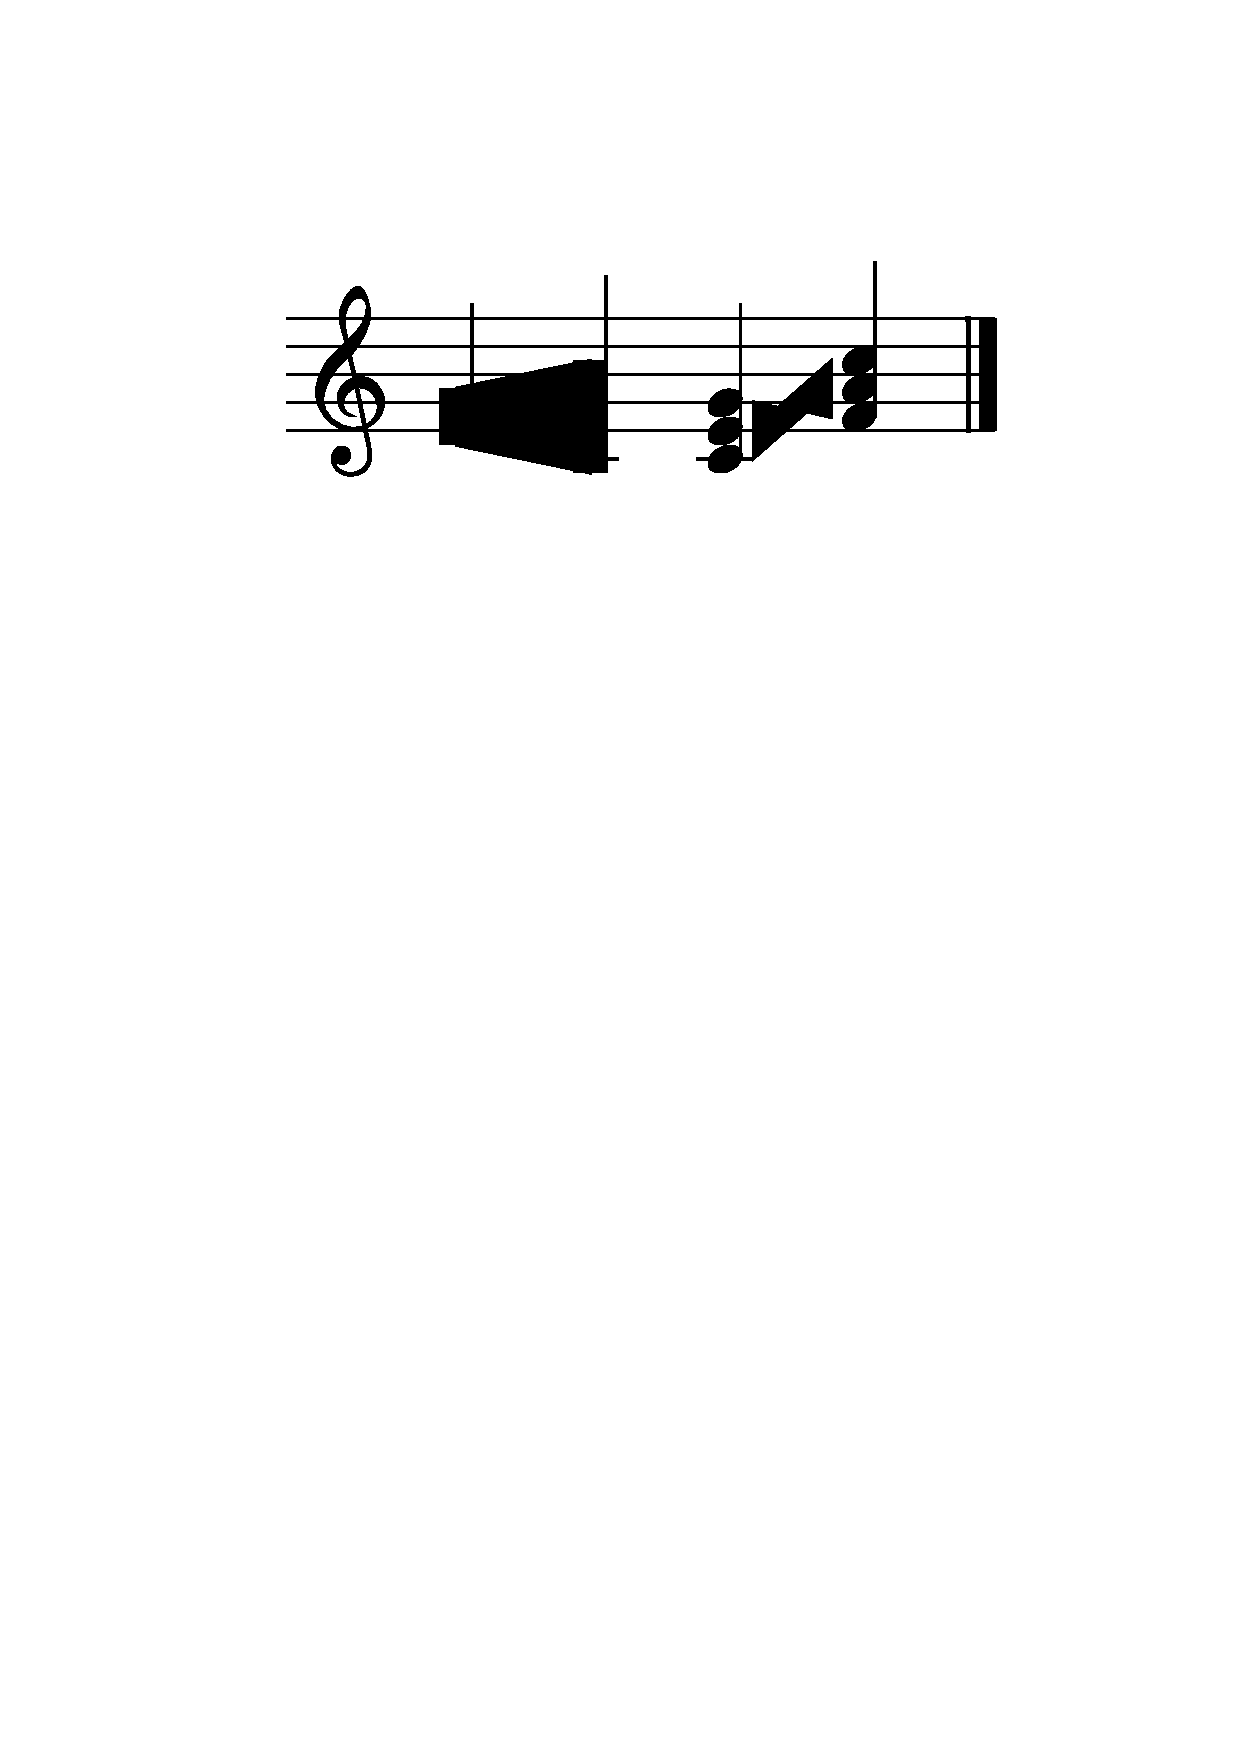
\includegraphics[width=55mm]{img/glissandofill.pdf}
\caption{glisandi entre accords et clusters avec option de remplissage}
\label{fig:glissandofill}
\end{center}
\end{figure}

\newpage

% *****************STAFFOFF/ON**********************
\subsection{Tags staffOff / staffOn}

\begin{code}
[ ... \textbackslash{}staffOff ... \textbackslash{}staffOn ... ]
\end{code}
\\

% littérature ?????????????
% lilypond : même principe, mais les notes et autres éléments se dessinent dans le vide
% permet aussi de passer d'un style de portée à un autre (override staff) ex : 2 lignes...

L'implémentation de ce tag vient du besoin de pouvoir faire disparaître et apparaître la partition, en particulier pour cacher une voix muette pendant un certain temps, et donc inutilement dessinée. (Figure \ref{fig:staffoffsimple}) 

Il est cependant généralisé à tous les éléments et toutes les voix de la partition et peut donc être utilisé à la guise et selon les fantaisies de l'utilisateur. (Figure \ref{fig:staffoffexotique})

\begin{figure}[h]
\centering
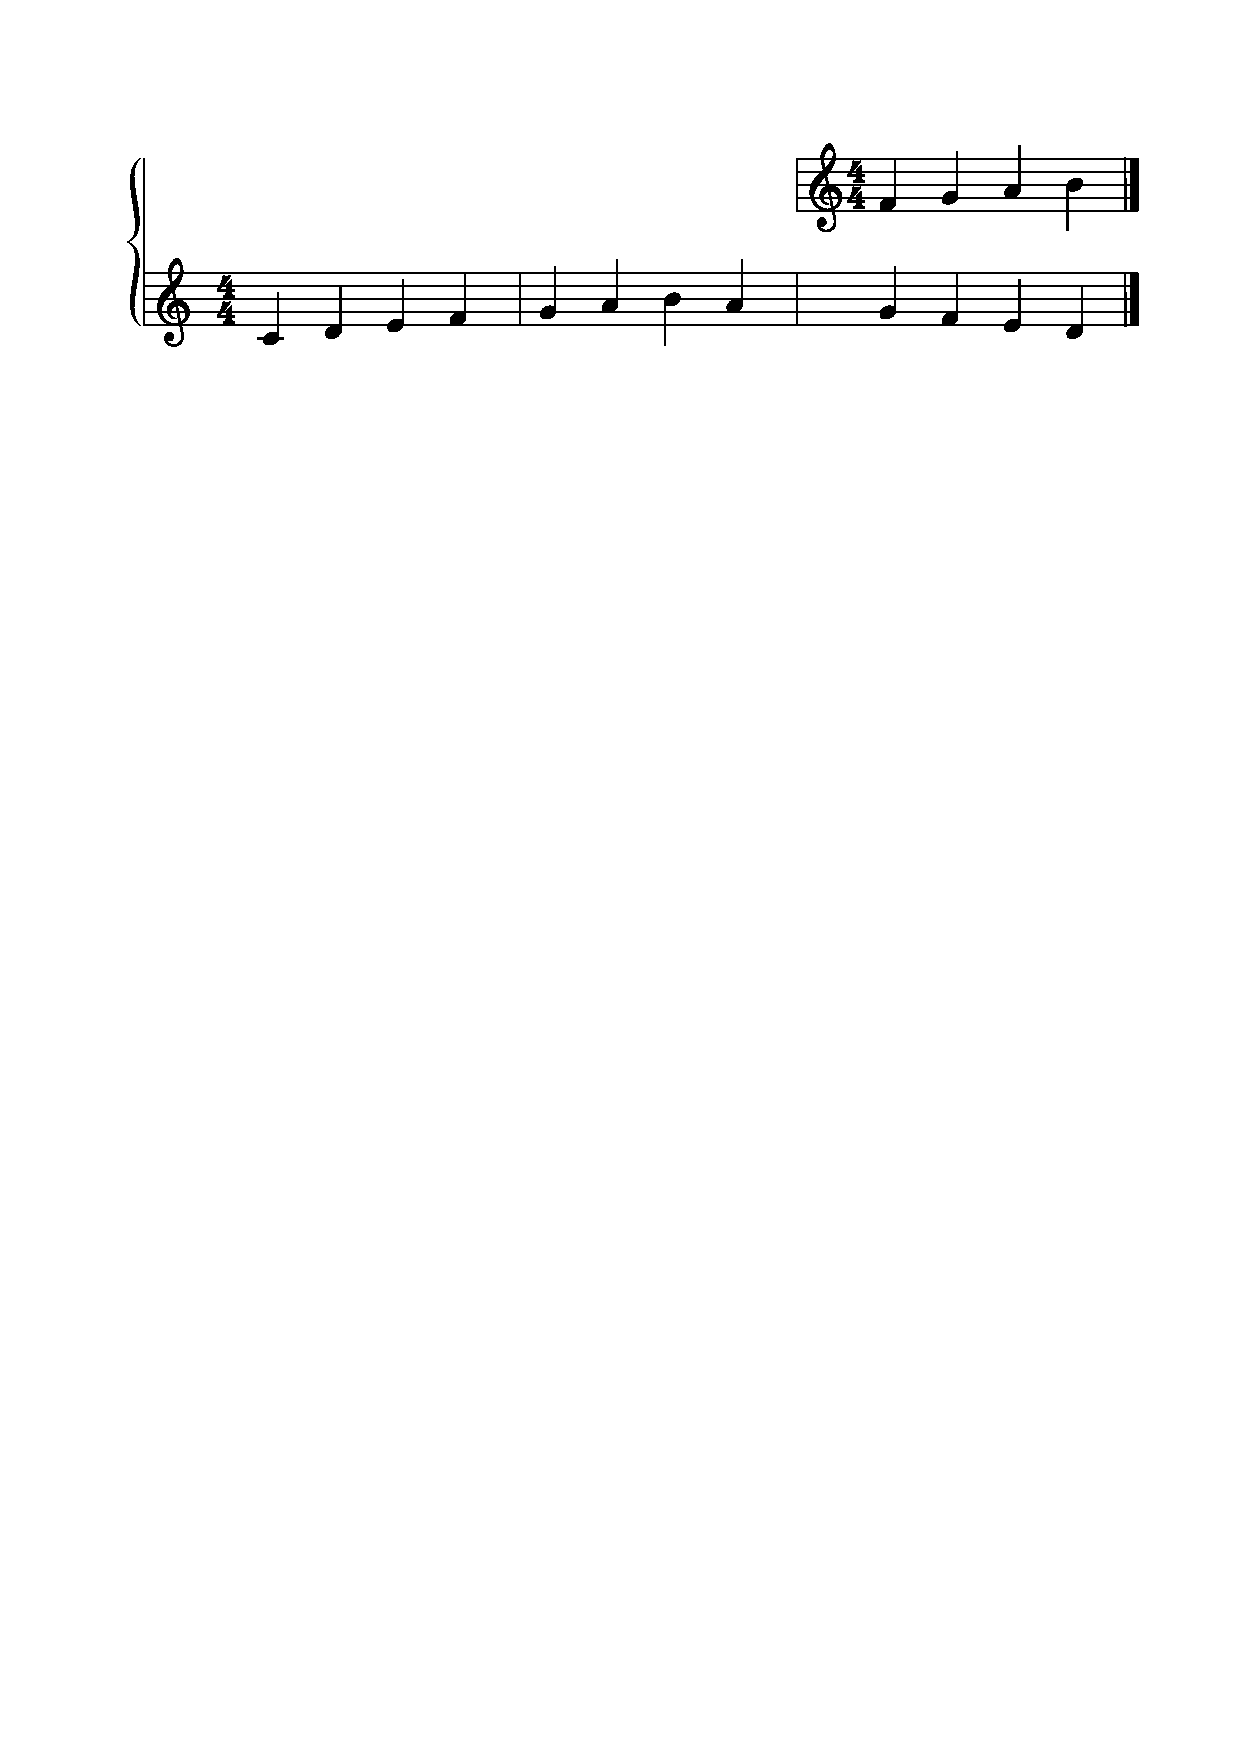
\includegraphics[width=8cm]{img/staffoff.pdf}
\caption{ Exemple staffOff classique}
\label{fig:staffoffsimple}
\end{figure}

%{[\meter<"3/4"> a b/2 c \staffOff g/4 e _\staffOn e a/2 \staffOff \slur(e g) \staffOn a b/4 ], [\meter<"3/4"> \staffOff \clef e \staffOn d g \staffOff _/2 g e g \staffOn a b g d/4]}

\begin{figure}[h]
\centering
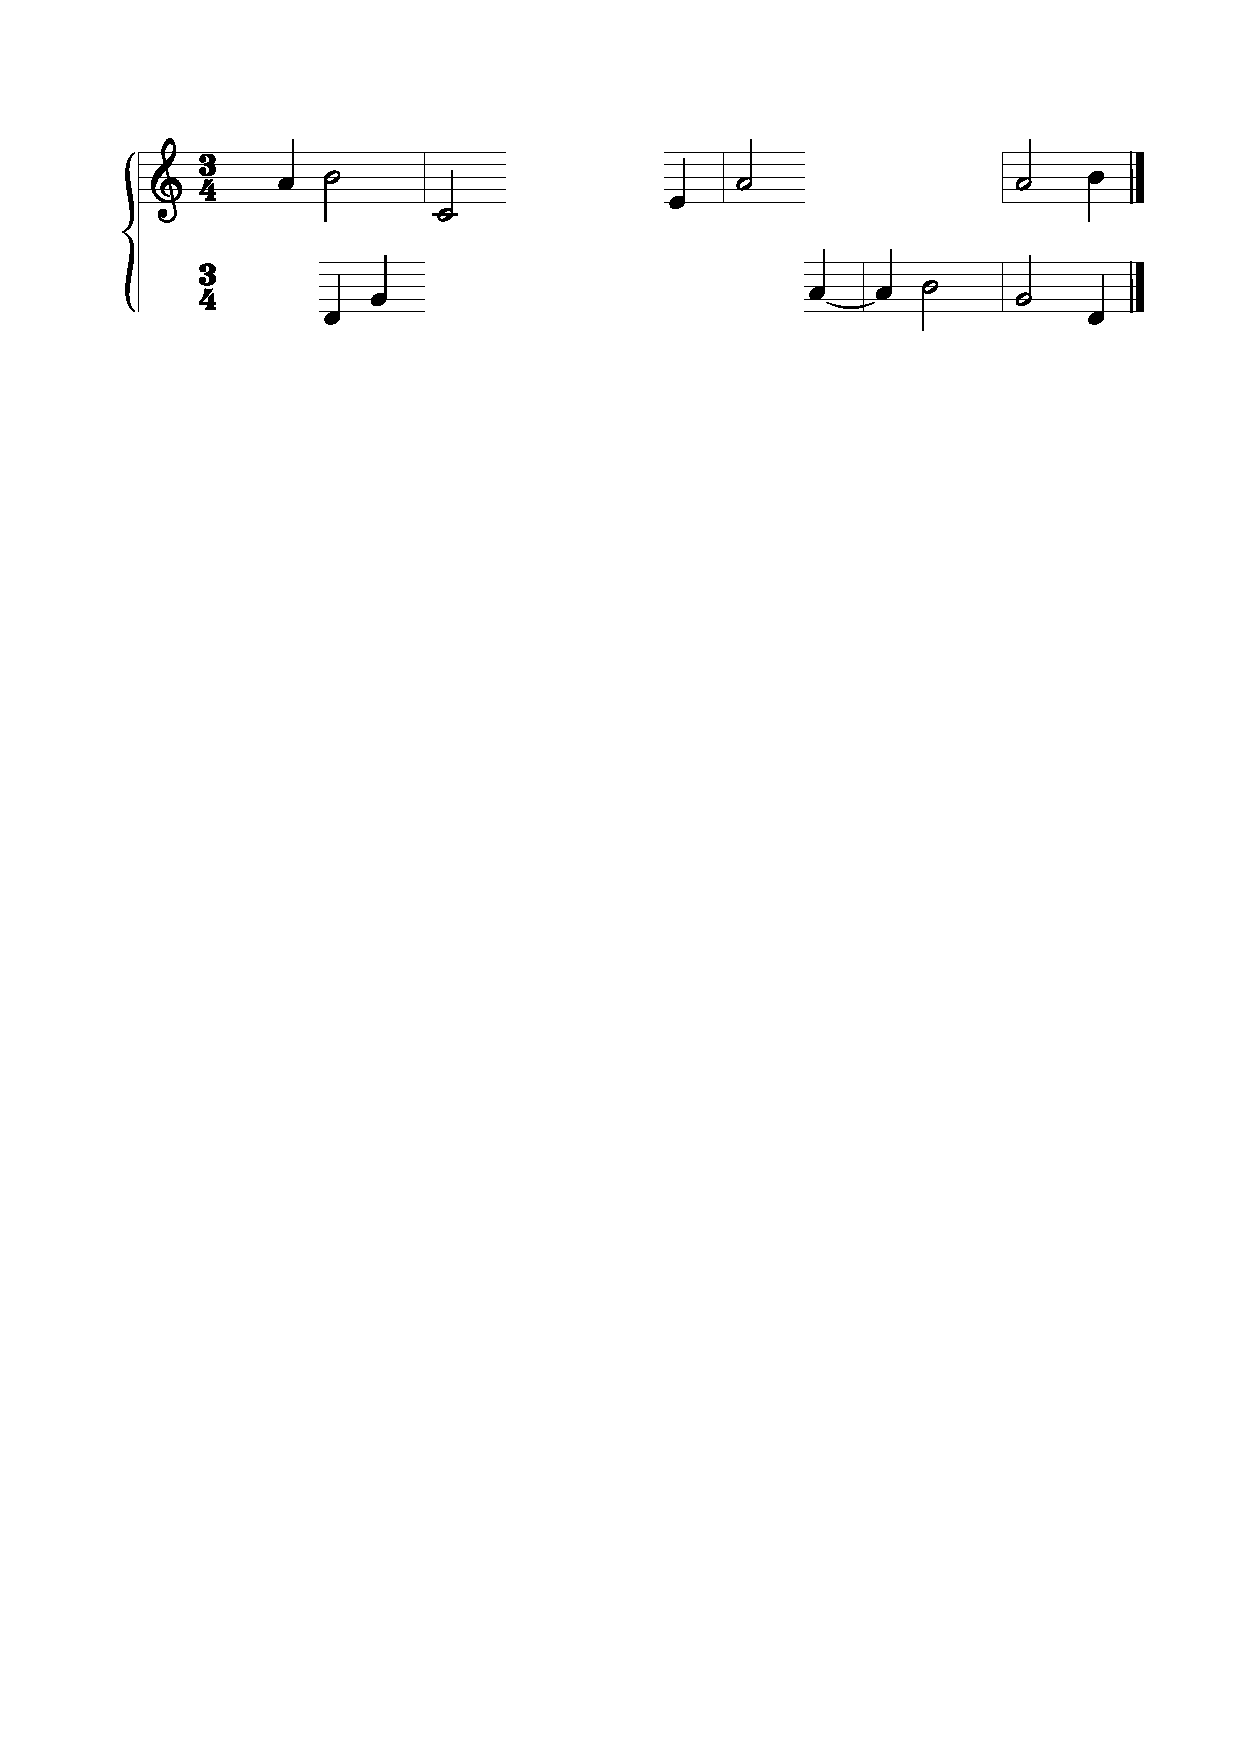
\includegraphics[width=8cm]{img/staffoffexotique.pdf}
\caption{ Exemple staffOff plus complexe}
\label{fig:staffoffexotique}
\end{figure}

Il fut important de définir les positions temporelles et graphiques correspondant aux positions dans la description textuelle, en particulier pour les éléments sans durée, dont la position était la même que le tag. La solution implémentée consiste à faire disparaître tous les éléments inscrits après le tag \textbackslash{}staffOff dans la description textuelle, et à préserver ceux décrits avant, même dans le cas d'éléments de durée nulle qui donc pourraient être considérés simultanés à l'arrivée du tag. Pour plusieurs éléments simultanés, c'est donc bien l'ordre dans la description textuelle qui indiquera le comportement à adopter. Ainsi, écrire % exemple utile ? pertinent sans image ?

\begin{center}
\begin{code}
[\textbackslash{}meter\textless{}"4/4"\textgreater{} \textbackslash{}clef \textbackslash{}staffOff a b c \textbackslash{}staffOn d ]
\end{code}

n'est pas équivalent à écrire 
\\
\bigskip
\begin{code}
[\textbackslash{}staffOff \textbackslash{}meter\textless{}"4/4"\textgreater{} \textbackslash{}clef a b c \textbackslash{}staffOn d]
\end{code} 
\end{center}

Quant à la portée, elle commence, ou s'arrête, aux positions correspondant au début des éléments suivant le tag.

\newpage

%*****************SYMBOLES*****************************
\subsection{Symboles}

% colas /////////////

\newpage

% ***************** FEATHERED BEAM **********************
\subsection{Liens de croches en soufflet (feathered beaming)}

\begin{code}
\textbackslash{}fBeam\textless{}options\textgreater{}( croches )
\end{code}
\\

Décrite par Gardner Read dans son ouvrage "Music Notation. A Manual of Modern Practice" \cite{ref8} comme "a highly graphic representation of rythmic flexibility"(p.94), cette notation contemporaine d'un accelerando ou ritardando à travers les liens de croches est, de manière générale, encore peu répandue dans les ouvrages de théorie, et se résume souvent à des cas simples, partant ou arrivant à la simple croche, c'est à dire partant ou arrivant vers un unique point. Pourtant il paraît intéressant de pouvoir offrir la possiblité aux compositeurs de décrire le passage entre n'importe quelles valeurs : d'une double-croche à une triple-croche, ou d'une quadruple-croche à une double-croche... (Figure \ref{fig:fbeamcomplex})

\begin{figure}[h]
\centering
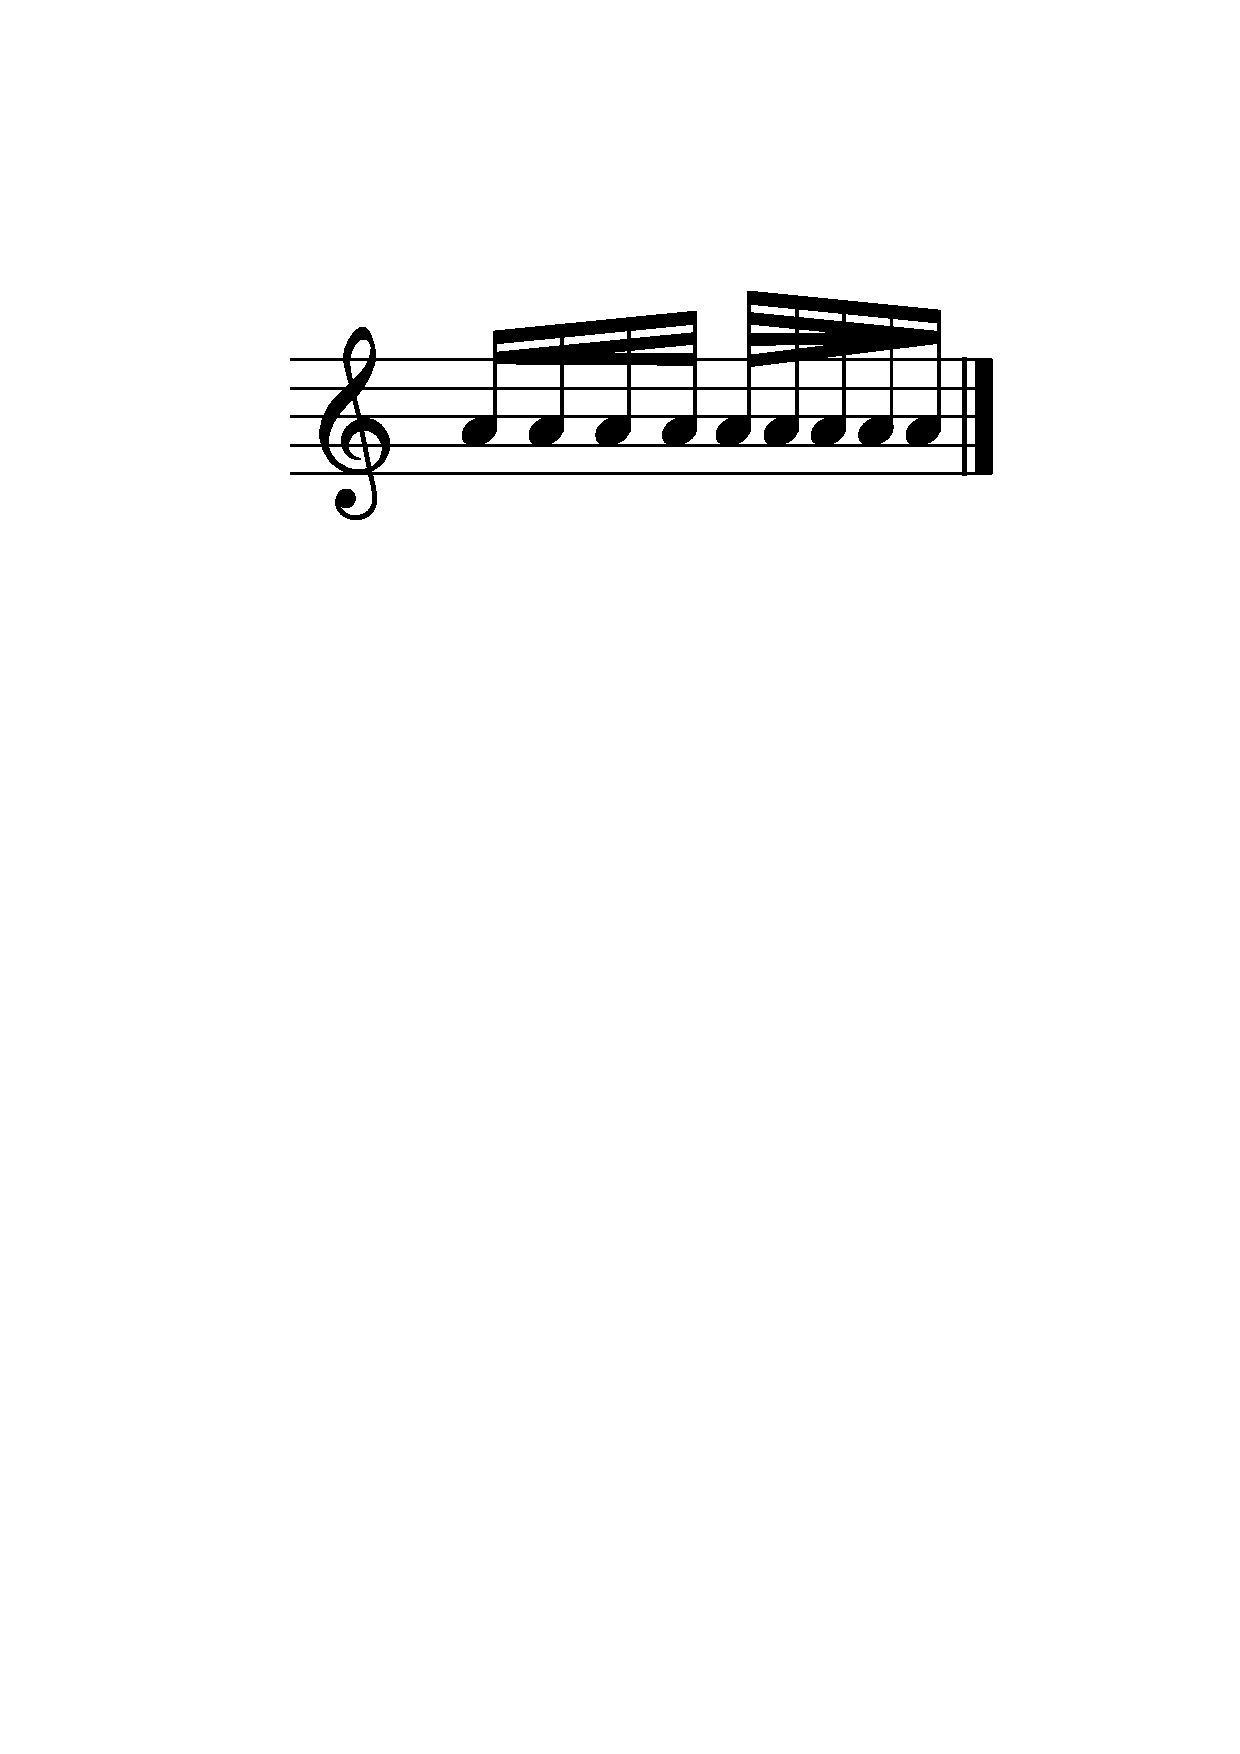
\includegraphics[width=6cm]{img/fbeamcomplex.pdf}
\caption{Exemple de feathered beams plus complexes}
\label{fig:fbeamcomplex}
\end{figure}

% question de voix simultanées
% lilypond : 
% \override Beam #'grow-direction = #LEFT
% \featherDurations #(ly:make-moment 2 1)
% { c16[ c c c c c c c] }

On remarque que, même dans un ouvrage tel que celui d'Elaine Gould \cite{ref2}, peu de détails sont donnés sur cette notation, et on se heurte rapidement à des incohérences telles que celle de la figure \ref{fig:incoherence} tirée de "Behind Bars" : on veut faire tenir en un temps une croche et quatre notes de durées inférieures à la croche mais supérieures à la triple-croche. 

\begin{figure}[h]
\centering
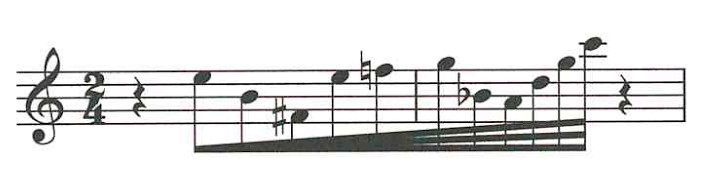
\includegraphics[width=7cm]{img/behindbars.jpg}
\caption{Exemple d'incohérence entre la durée totale et les durées individuelles des notes d'un groupe lié. (Behind Bars, p.158) }
\label{fig:incoherence}
\end{figure}

Ce manque d'une exacte cohérence entre tempo et aspect graphique est également souligné dans "Music Notation in the Twentieth Century" de Kurt Stone \cite{ref3} : "Besides, the gradual increase or decrease in the number of beams makes exact indications of beat-units impossible" (p.124).

Ainsi on voit l'importance des choix de design de ce symbole, sur la manière de le décrire textuellement, de le dessiner en particulier dans le cas de plusieurs voix simultanés, et de manière générale sur la liberté laissée à l'utilisateur.
\\

Concernant les possibilités de description données à l'utilisateur. Nous avons vu que plusieurs critères pouvaient intervenir dans la description, et devaient pouvoir être imposés par l'utilisateur. Des paramètres qui peuvent être incohérents entre eux :
\begin{itemize}
\item le nombre de notes dans le groupe,
\item leurs durées individuelles et intrinsèques qui définissent également leur espacement,
\item la durée totale du groupe, dépendante directement des durées individuelles,
\item les durées de départ et d'arrivée qui définissent l'aspect graphique du feathered beam.
\end{itemize}

Ces différents niveaux de description nous poussent à faire une claire distinction entre l'aspect temporel et l'aspect graphique de notre groupe de notes.  Il a été décidé de laisser au compositeur la liberté de donner à son feathered beam l'aspect graphique qu'il désire, indépendamment des durées internes de ses notes. Il pourra ainsi jouer sur les espacements entre notes, sur le nombre de notes, et sur la durée totale de manière "classique" en imposant à chaque note une durée, et en veillant à ce que la somme de toutes les notes corresponde à la durée totale souhaitée. Cette durée totale peut être indiquée sur la partition grâce au paramètre \textit{drawDuration} (Figure \ref{fig:fbeamduree}).

\begin{figure}[h]
\centering
\begin{code}
[ \textbackslash{}fBeam\textless{}drawDuration="true"\textgreater{}

( a/8 a a/16 a a a/32 a ) ]
\end{code}
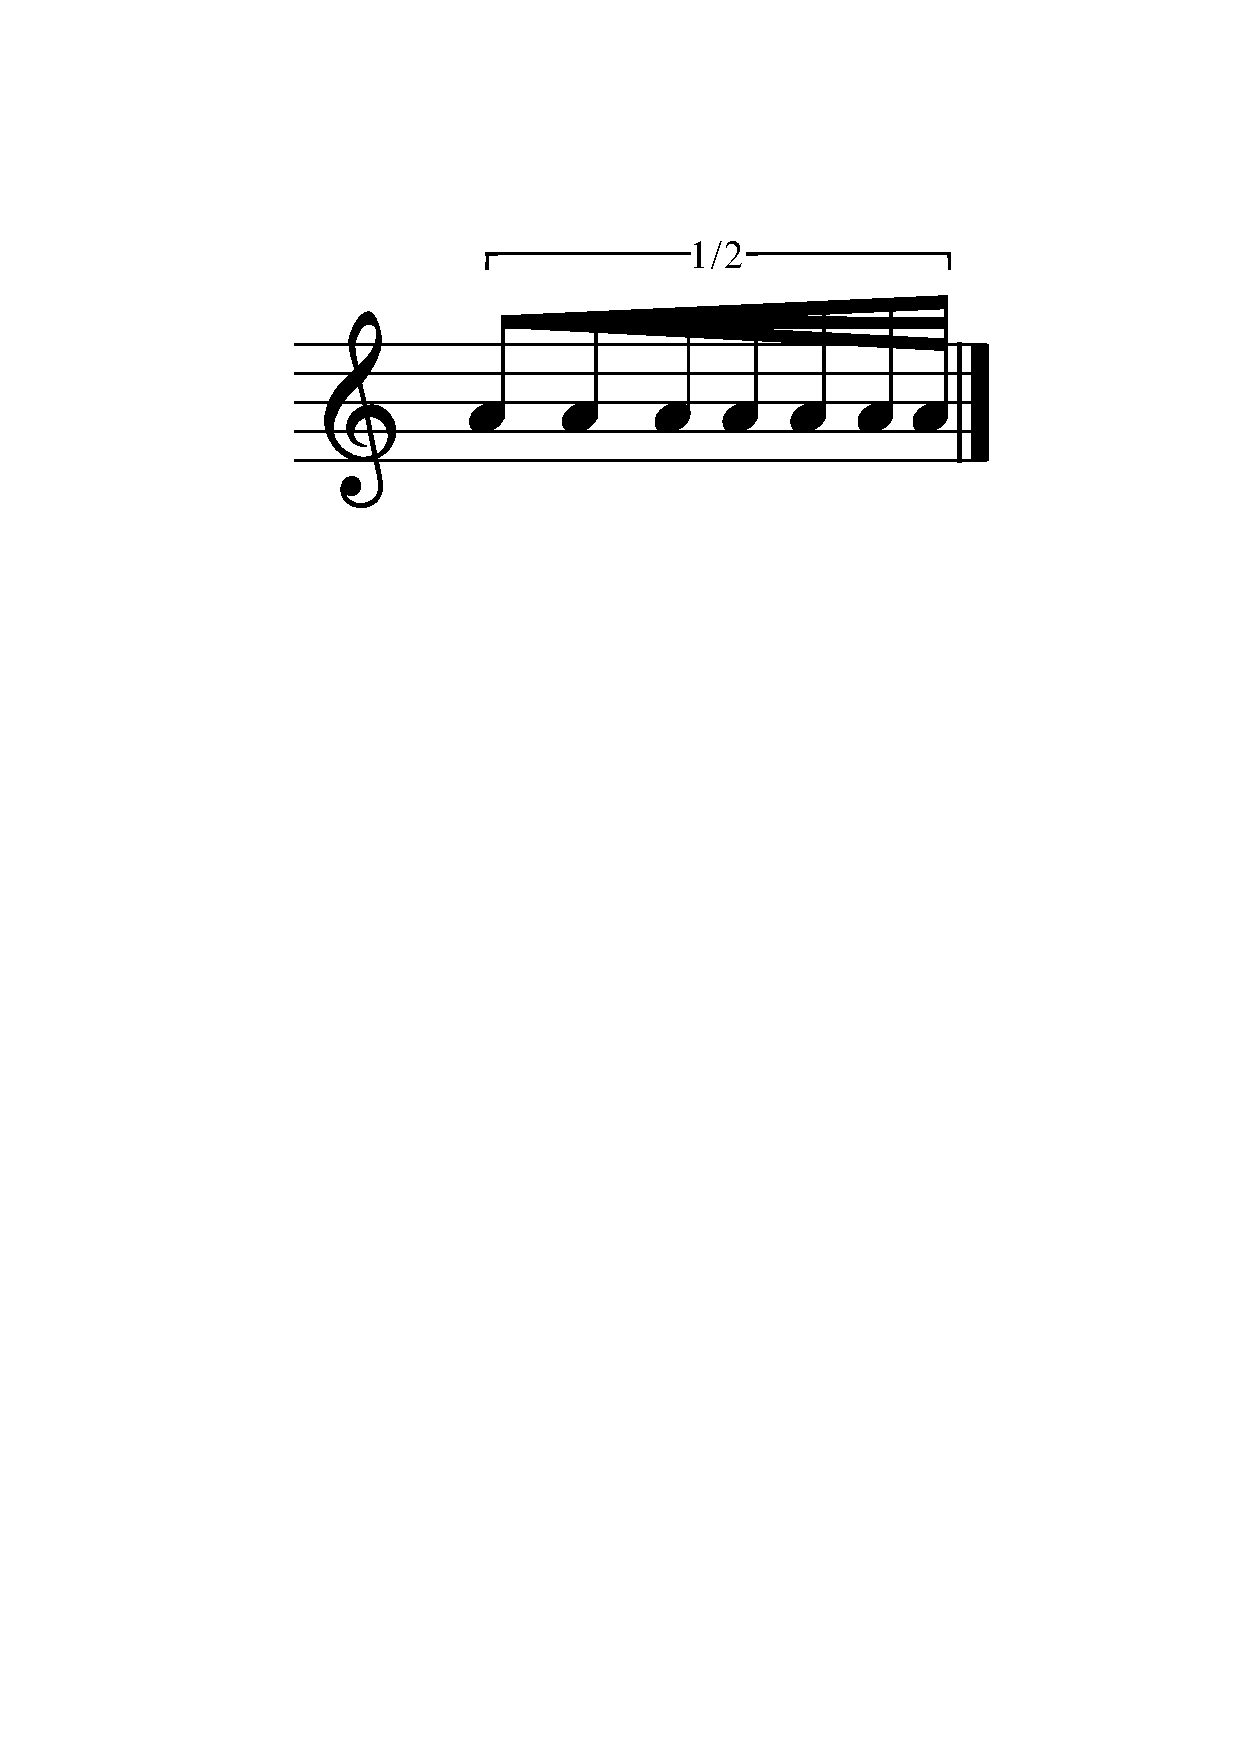
\includegraphics[width=6cm]{img/fbeamduree.pdf}
\caption{Représentation de la durée}
\label{fig:fbeamduree}
\end{figure}

Sans plus d'indication de sa part, l'aspect graphique suivra les durées réelles des notes et prendra comme points de départ et d'arrivée les durées des première et dernière notes.  C'est le cas de la Figure \ref{fig:fbeamduree}.

En revanche, le paramètre \textit{durations} pourra lui permettre d'imposer un aspect graphique tout autre, lui donnant ainsi la possibilité d'indiquer à l'interprète un changement de tempo plus ou moins important, pas forcément cohérent avec les durées intrinsèques des notes, mais ayant du sens dans l'interprétation (Cf Figure \ref{fig:utilisateur}).

\begin{comment}
Ainsi, les deux descriptions suivantes sont valides, mais pas équivalentes :
\\

\begin{figure}[h]
\centering
\begin{code}
[ \textbackslash{}fBeam\textless{}drawDuration="true"\textgreater{}

 (a/16 a a a/32 a/64 a) ]
\end{code}

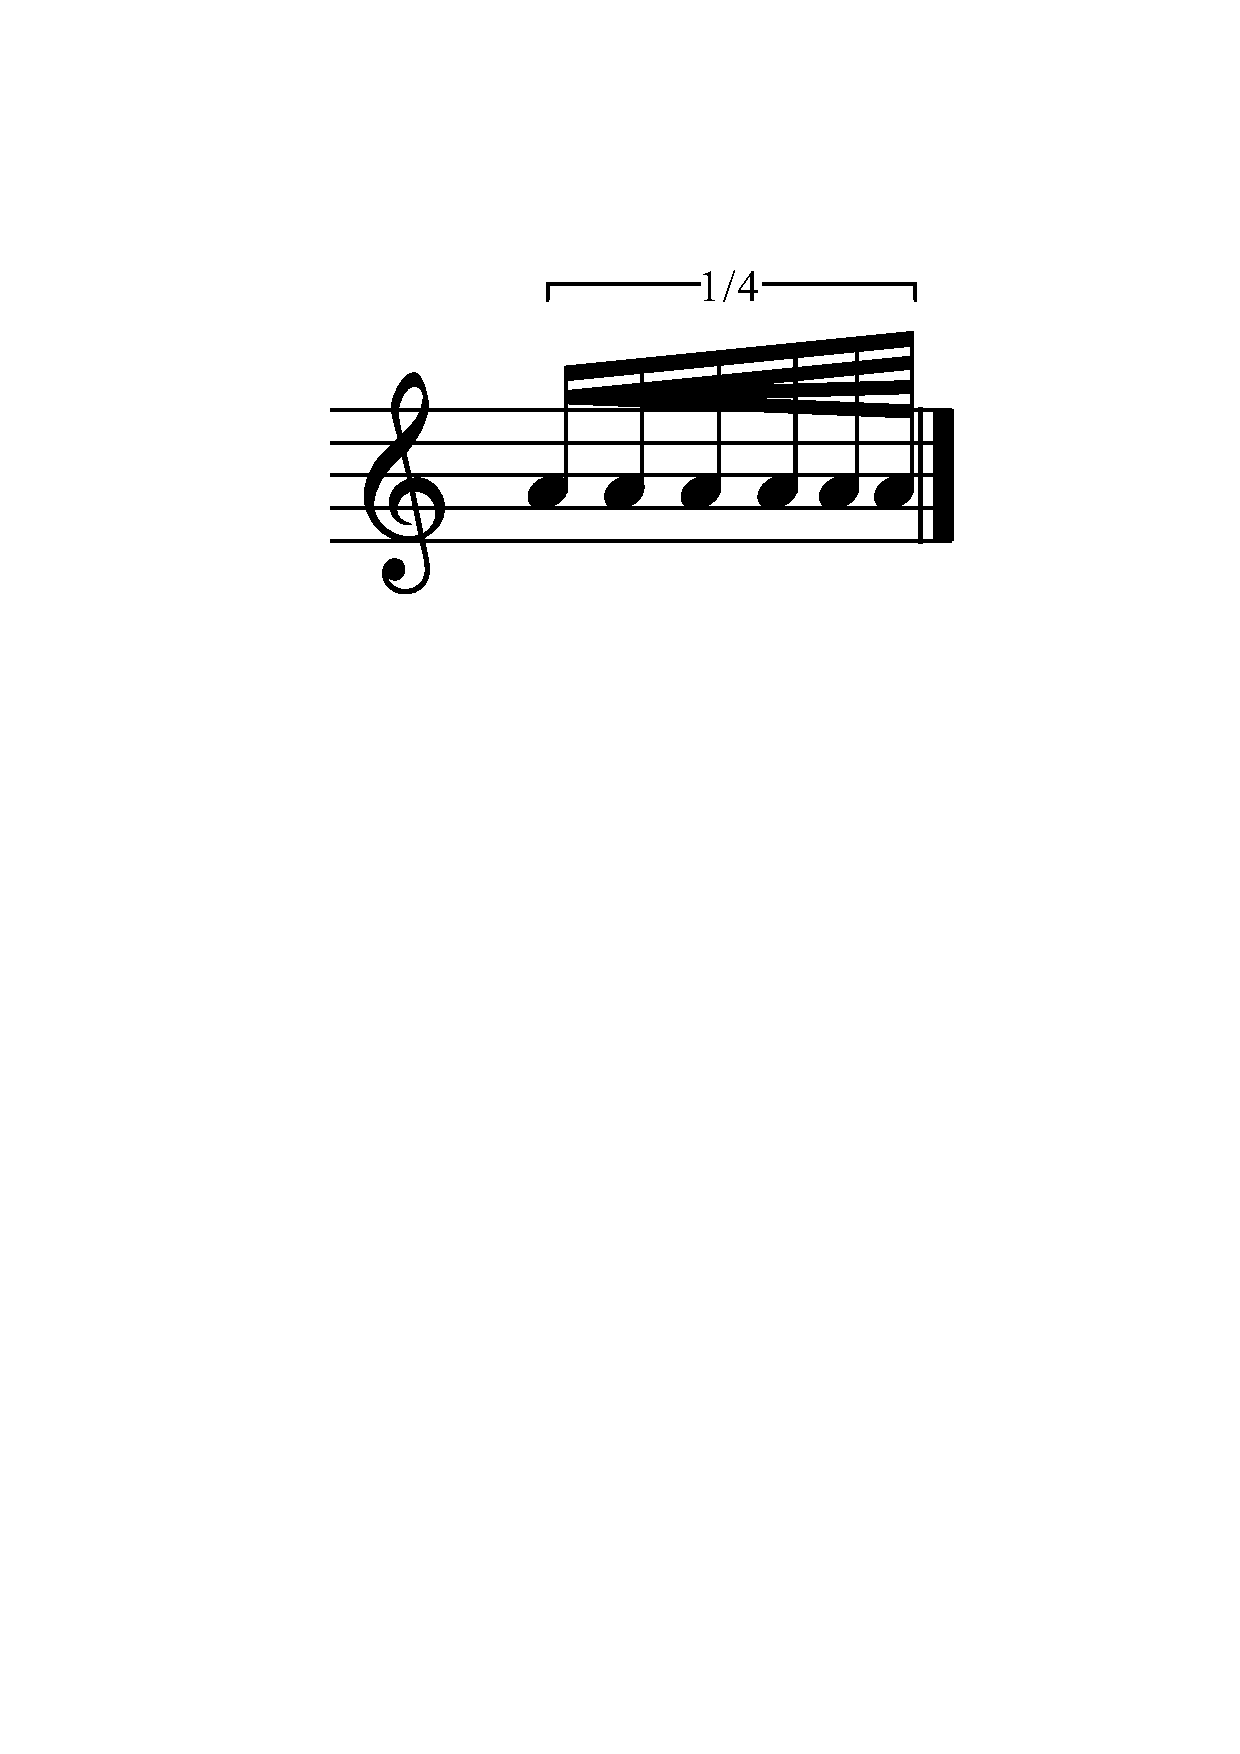
\includegraphics[width=5cm]{img/durationsinternes.pdf}
\caption{Aspect graphique imposé par les durées internes}
\label{fig:interne}
\end{figure}
\end{comment}

\begin{figure}[h]
\centering
\begin{code}
[ \textbackslash{}fBeam\textless{}durations="1/16,1/64", drawDuration="true"\textgreater{}(a/8 a/16 a a a/32 a) ]
\end{code}

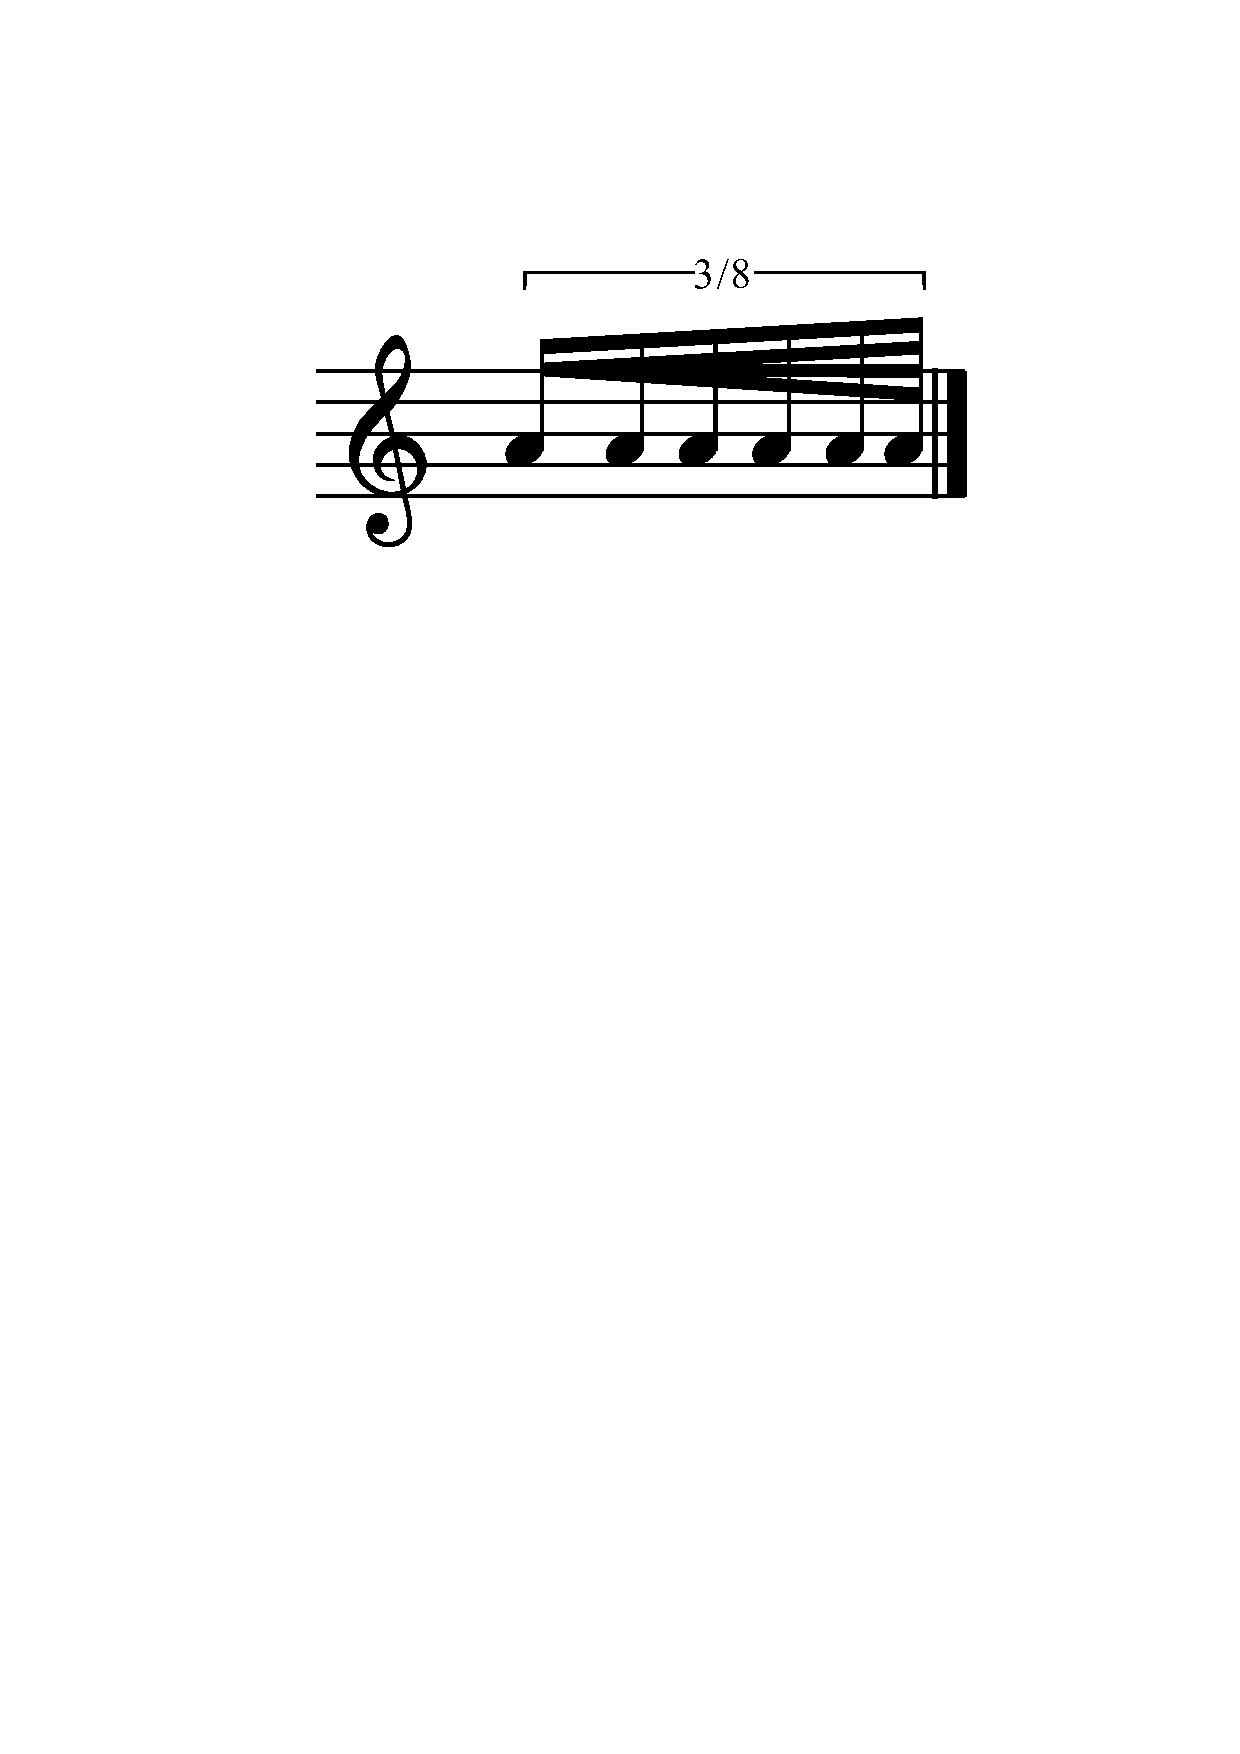
\includegraphics[width=5cm]{img/durations.pdf}
\caption{Aspect graphique imposé par l'utilisateur}
\label{fig:utilisateur}
\end{figure}

Dans un désir de simplicité, il a été décidé de décrire par un seul tag un seul groupe de notes liées, correspondant à un point de départ et un point d'arrivée uniques. Il est cependant possible de chaîner plusieurs feathered beams grâce à la faculté du tag à se séparer en \textbackslash{}fBeamBegin et \textbackslash{}fBeamEnd, permettant alors, non seulement de chaîner deux beams par une note (Figure \ref{fig:fbeamchain}), mais de les faire se chevaucher sur plusieurs notes.

\begin{figure}[h]
\centering
\begin{code}
[ \textbackslash{}fBeamBegin :1 c/8 d e/16 \textbackslash{}fBeamBegin :2 f/32 \textbackslash{}fBeamEnd :1 e/16 d/8 c
\textbackslash{}fBeamEnd :2 ]
\end{code}
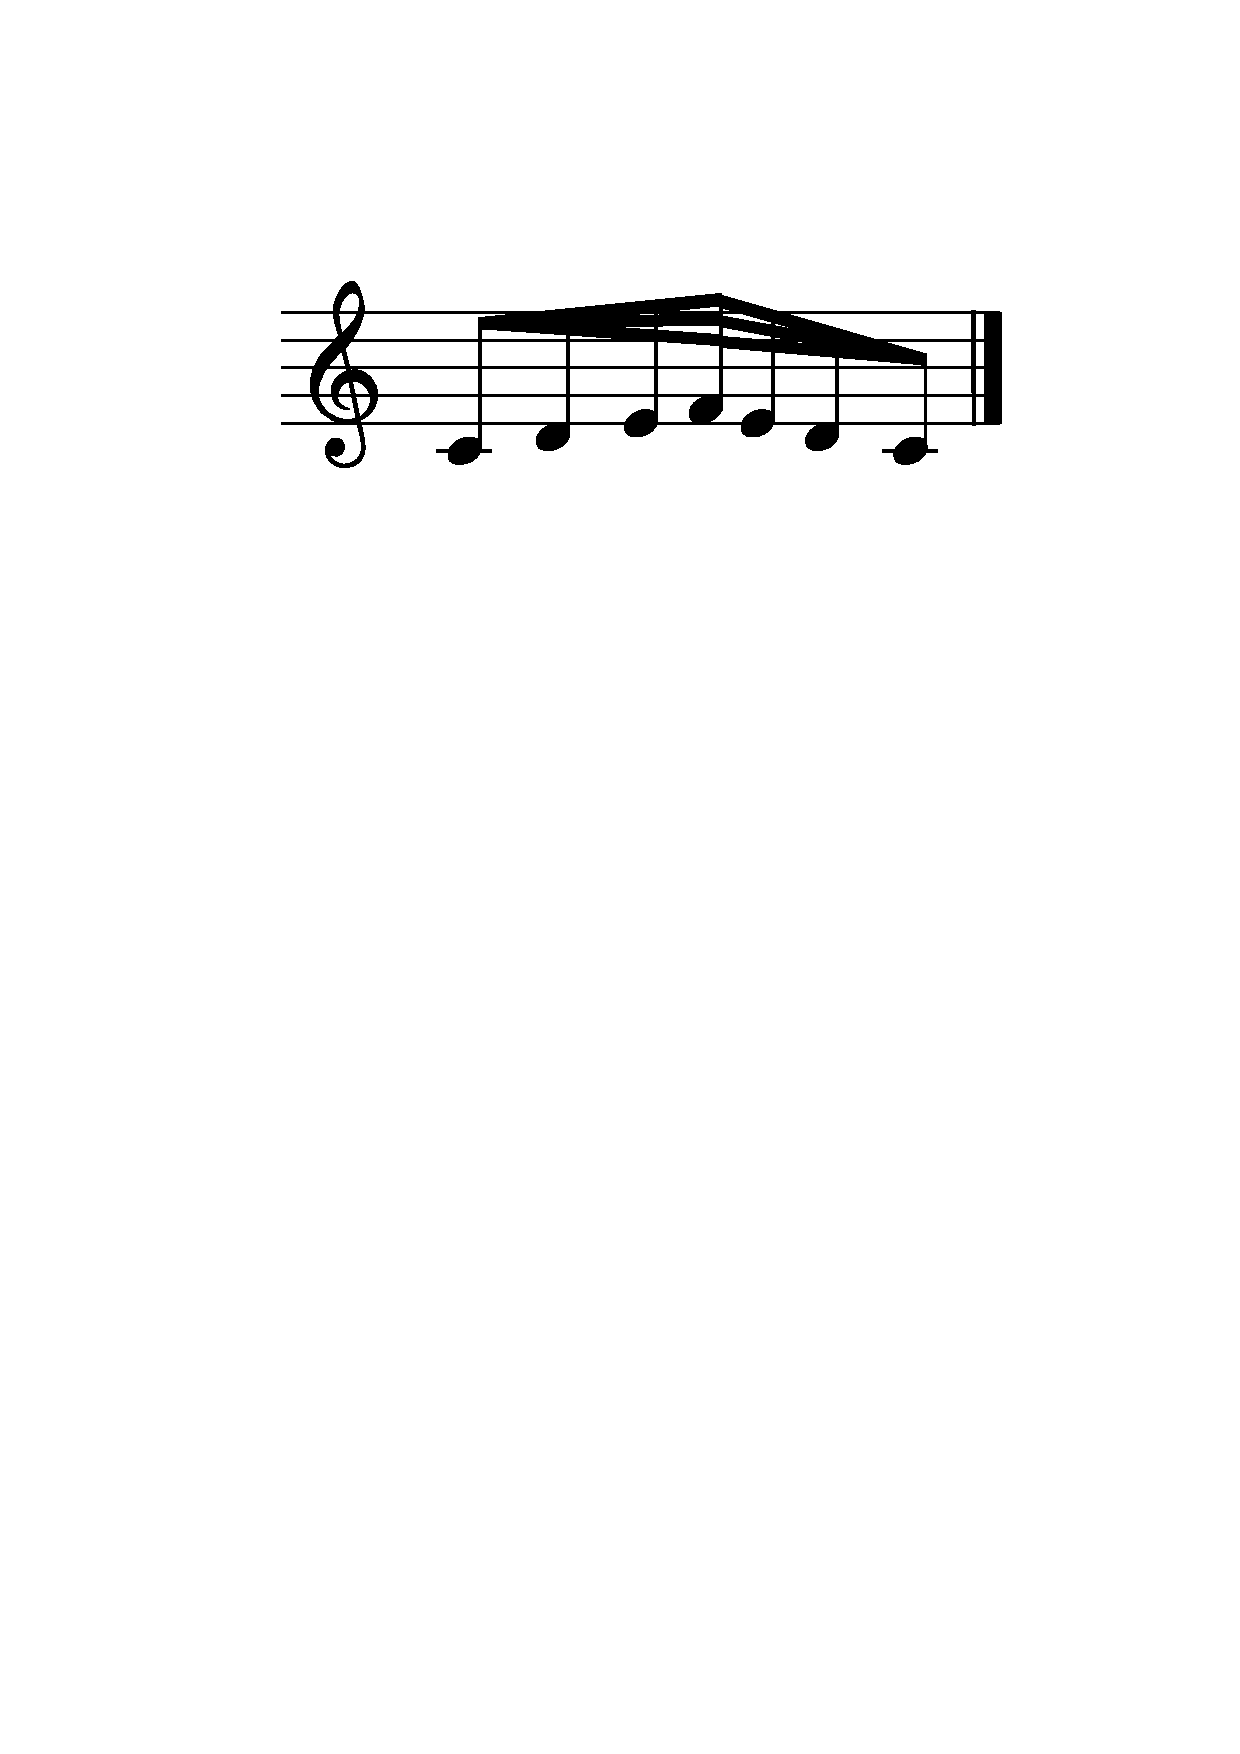
\includegraphics[width=6cm]{img/fBeamChaine.pdf}
\caption{Feathered beams chaînés}
\label{fig:fbeamchain}
\end{figure}

% justification des hierarchies de beams ?
Enfin, concernant le feathered beam comme le beam classique, il est maintenant possible de créer des hierarchies de beams : c'est à dire d'englober plusieurs beams dans un plus grand, afin de les joindre par une barre principale commune (Figure \ref{fig:fbeamhierarchie}).

\begin{figure}[h]
\centering
\begin{code}
[ \textbackslash{}beam( \textbackslash{}fBeam(c/8 e d f g/32) 

\textbackslash{}fBeam(a/16 f e d c/64) ) ]
\end{code}

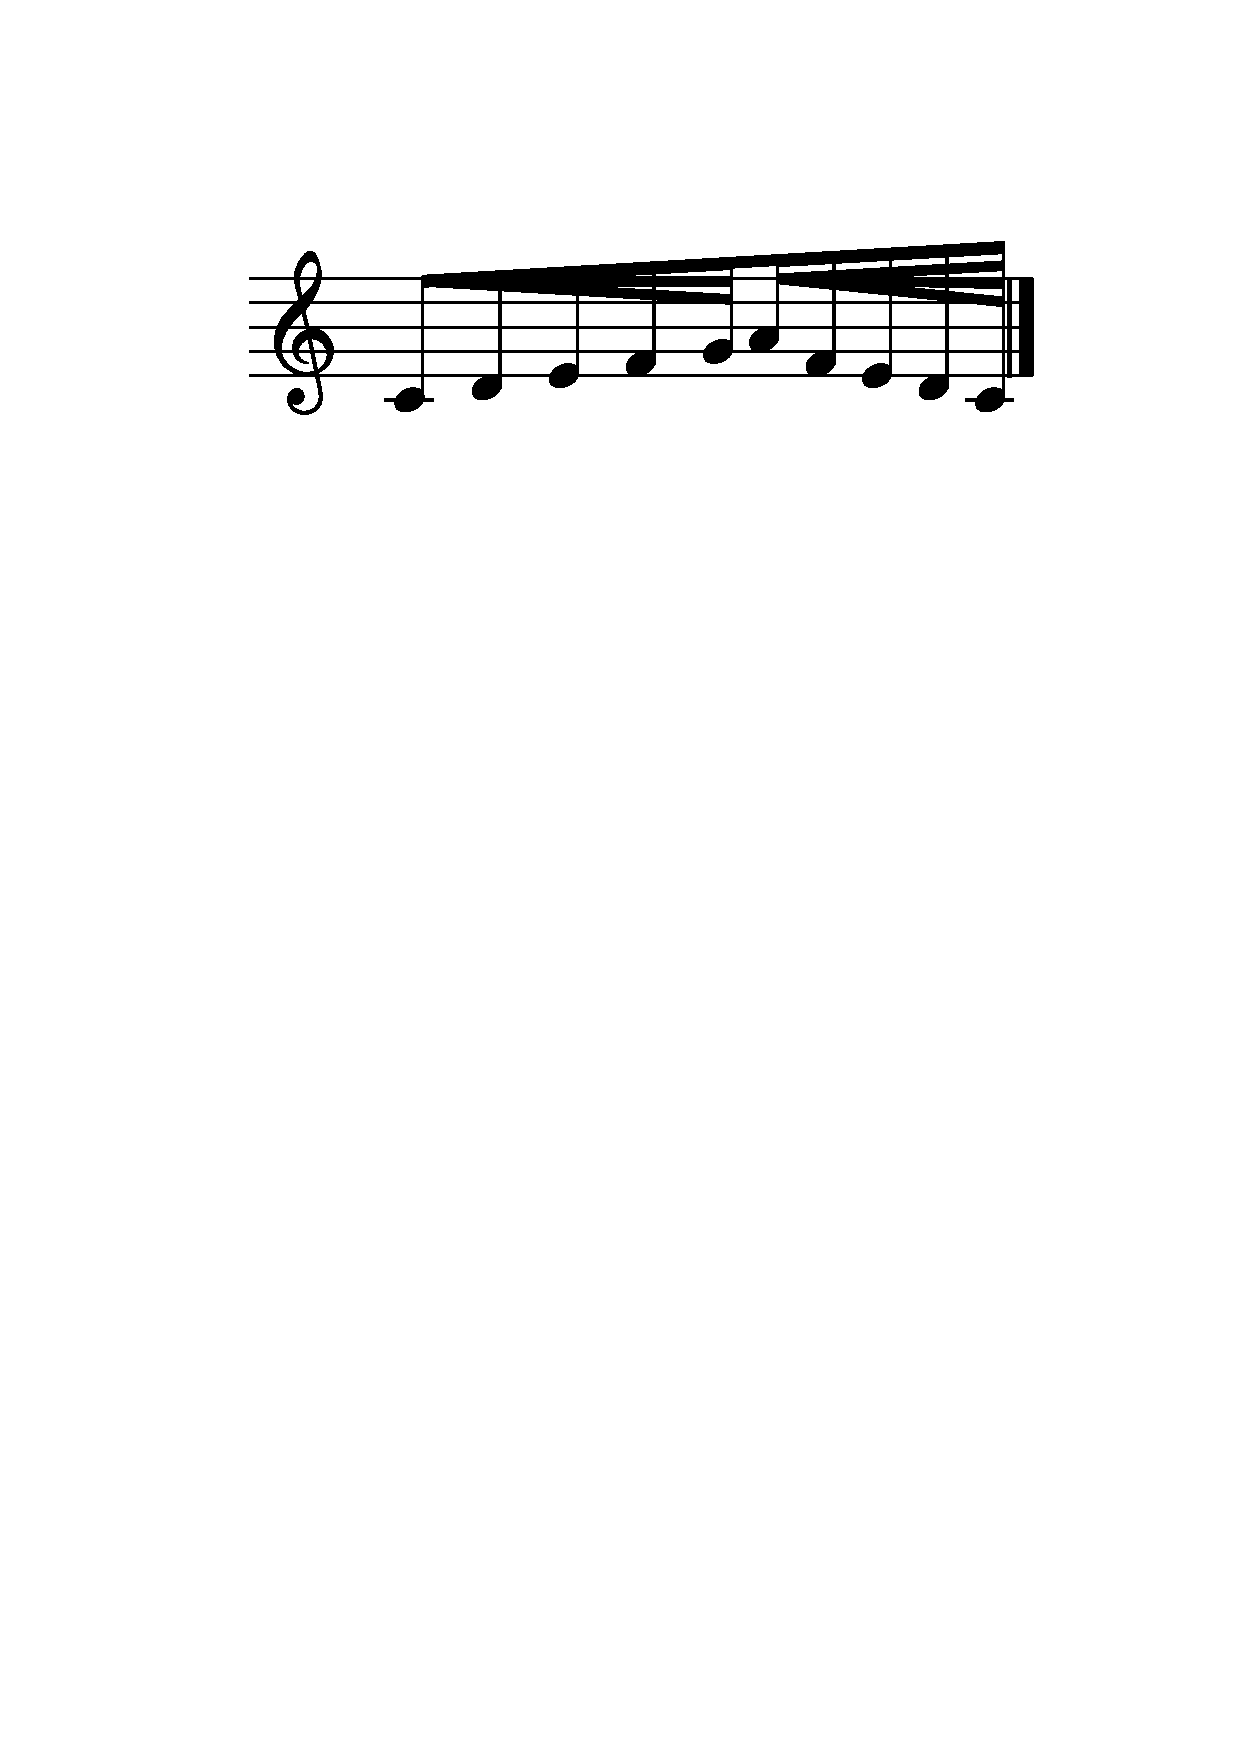
\includegraphics[width=6cm]{img/fBeamHierarchie.pdf}
\caption{Feathered beams englobés dans un plus grand}
\label{fig:fbeamhierarchie}
\end{figure}

%*********************COMBINAISONS********************
\section{Combinaisons}
% exemples de "vraies" oeuvres de compositeurs ?

%*********************CONCLUSION**********************
\section{Conclusion}

% a faire /////////////////////////////////////////////////////

\bibliographystyle{plain}
\bibliography{publication}


\end{document}

